\section{Historical Evolution: From Parallel to Serial}
The evolution of computer input/output (I/O) interconnects has been driven by the relentless demand for higher bandwidth, lower latency, and greater scalability. For decades, the dominant paradigm for connecting peripheral devices to the Central Processing Unit (CPU) was the parallel bus architecture. In this topology, multiple data bits are transmitted simultaneously across parallel wires synchronized to a single common clock.
However, as processor speeds increased exponentially in the late 1990s and early 2000s, the physical limitations of parallel buses began to create a significant bottleneck in system performance. To overcome these barriers, the industry underwent a fundamental paradigm shift, moving away from wide, parallel shared buses toward high-speed, point-to-point serial links. This transition laid the foundation for modern interconnect standards, including the Peripheral Component Interconnect Express (PCIe).
\section{The AI Revolution and the Scaling Imperative of PCIe Infrastructure}
The rise of artificial intelligence (AI) and Generative Al are transforming how we interact with technology. From 
healthcare to business efficiency and groundbreaking research, AI and Generative AI are making waves. These AI 
marvels rely on vast amounts of hardware and infrastructure to function. As such, data centers are undergoing a 
revolution driven by the ever-growing demands and workloads required to train AI and Generative AI. PCI Express 
technology is the workhorse of data center communication by offering high bandwidth, low latency, efficient data 
exchange between CPUs, GPUs, and other components. Today, PCIe has become the industry standard for 
connecting devices such as graphics cards, network adapters, and storage drives, enabling faster data transfer and 
more efficient system performance 



\section{PCIe Standards Overview}
Peripheral Component Interconnect Express (PCIe) is a high-speed serial computer expansion bus standard designed to replace the older PCI, PCI-X, and AGP bus standards. It is structured as a layered protocol, similar to the Open Systems Interconnection (OSI) model, which ensures modularity and scalability.
The PCIe architecture consists of three primary layers:
\begin{enumerate}
    \item \textbf{Transaction Layer}: Handles the assembly and disassembly of Transaction Layer Packets (TLPs). It manages flow control and ensures reliable delivery of packets.
    \item \textbf{Data Link Layer}: Ensures data integrity by adding error detection codes (LCRC) and managing the re-transmission of corrupted packets (via ACK/NAK protocols).
    \item \textbf{Physical Layer (PHY)}: The focus of this thesis, this layer is responsible for the electrical interface, serialization, de-serialization, and clock recovery. It converts the digital packets into analog differential signals suitable for transmission across the physical medium.
\end{enumerate}

\subsection{Evolution of PCIe}
Since its inception, the PCIe standard has undergone continuous evolution to meet the bandwidth demands of modern computing. The data rate has approximately doubled with each generation, maintaining backward compatibility while introducing more efficient encoding schemes.

The evolution of the standard can be categorized by the modulation and encoding techniques employed:

Gen 1.0 (2.5 GT/s) \& Gen 2.0 (5.0 GT/s): The initial generations utilized Non-Return-to-Zero (NRZ) signaling with 8b/10b encoding. This encoding scheme mapped 8 bits of data to 10 bits of transmitted symbols to ensure DC balance and sufficient transition density for clock recovery. However, this introduced a 20\% overhead, reducing the effective throughput.

Gen 3.0 (8.0 GT/s), Gen 4.0 (16.0 GT/s) \& Gen 5.0 (32.0 GT/s): To improve efficiency, Gen 3.0 introduced 128b/130b encoding. This drastically reduced the overhead from 20\% to approximately 1.5\%, allowing for higher effective data rates without proportionally increasing the clock frequency. These generations continued to use NRZ signaling, where the Nyquist frequency is half the data rate (e.g., 16 GHz for Gen 5).

Gen 6.0 (64.0 GT/s): This generation marks a revolutionary shift in the standard. To achieve 64 GT/s without requiring unreasonable channel bandwidths (which would exceed 32 GHz), the standard moved from 2-level NRZ modulation to 4-level Pulse Amplitude Modulation (PAM4).

PAM4 Signaling: Instead of transmitting 1 bit per Unit Interval (UI), PAM4 transmits 2 bits per UI using four distinct voltage levels. This effectively doubles the data rate while maintaining the same Nyquist frequency (16 GHz) as PCIe Gen 5.0.

Forward Error Correction (FEC): Due to the reduced Signal-to-Noise Ratio (SNR) inherent in PAM4 (the eyes are 1/3 the height of NRZ), Gen 6.0 mandates the use of lightweight Forward Error Correction (FEC) and Flow Control Unit (FLIT) encoding to maintain low Bit Error Rates (BER).
\begin{table}[htbp]
    \centering
    \caption{Comparative Analysis of PCIe Generations 3.0-6.0}
    \label{tab:pcie_comparison}
    \begin{tabular}{|l|l|l|l|l|}
        \hline
        \textbf{Feature} & \textbf{PCIe 3.0} & \textbf{PCIe 4.0} & \textbf{PCIe 5.0} & \textbf{PCIe 6.0} \\ \hline
        \textbf{Data Rate} & 8.0 GT/s & 16.0 GT/s & 32.0 GT/s & \textbf{64.0 GT/s} \\ \hline
        \textbf{Nyquist Freq} & 4 GHz & 8 GHz & 16 GHz & \textbf{16 GHz} \\ \hline
        \textbf{Encoding} & 128b/130b & 128b/130b & 128b/130b & \textbf{1b/1b FLIT} \\ \hline
        \textbf{Signaling} & NRZ & NRZ & NRZ & \textbf{PAM4} \\ \hline
        \textbf{Unit Interval} & 125 ps & 62.5 ps & 31.25 ps & \textbf{31.25 ps} \\ \hline
        \textbf{Channel Loss} & 20 dB & 28 dB & 36 dB & \textbf{32 dB} \\ \hline
    \end{tabular}
\end{table}
\subsection{PCIe 6.0 Standard Transmitter Specs}
\begin{table}[H]
    \centering
    \caption{Complete PCIe Gen 6 Transmitter (TX) Electrical Specifications}
    \label{tab:pcie6_tx_specs_full}
    \begin{tabular}{l l p{6cm}}
        \toprule
        \textbf{Spec} & \textbf{Value} & \textbf{Definition} \\
        \midrule
        $UI_{TX}$ & 31.246 -- 31.253 ps & Transition time (100 PPM)  \\
        $V_{TX-DIFF-PP}$ & 800 mV -- 1.0 V & Full swing diff. peak-to-peak  \\
        $V_{TX-DIFF-PP-LOW}$ & 400 mV -- 1.0 V & Low swing diff. peak-to-peak  \\
        $R_{LM}$ & 0.95 (min) & Level Separation Mismatch Ratio  \\
        $SNDR_{TX}$ & 34 dB (min) & Signal-to-Noise Distortion Ratio  \\
        $V_{TX-AC-CM-PP}$ & 25 mV (max) & AC peak-to-peak common mode  \\
        $V_{TX-AC-CM-PP-filt}$ & 75 mV (max) & Filtered AC common mode  \\
        $C_{TX}$ & 176 -- 265 nF & AC coupling capacitance  \\
        $Z_{TX-DIFF-DC}$ & 120 $\Omega$ (max) & DC Differential Impedance  \\
        $I_{TX-SHORT}$ & 90 mA (max) & Max transmitter short current  \\
        $T_{TX-UTJ}$ & 4.00 ps (max) & Uncorrelated total jitter  \\
        $T_{TX-UPW-TJ}$ & 4.00 ps (max) & Total uncorrelated pulse width jitter  \\
        $T_{TX-UPW-DJDD}$ & 1.25 ps (max) & Deterministic UPW jitter  \\
        $T_{TX-RJ}$ & 0.26 -- 0.42 ps & Random Jitter (RMS)  \\
        \bottomrule
    \end{tabular}
\end{table}
% ==================================================
% CHAPTER 2: Technology
% ==================================================
\chapter{GF 22nm FD-SOI technology}

\section{Planar MOSFET vs. SOI Technology}

The transition from conventional Planar MOSFETs to Silicon on Insulator (SOI) technology addresses several scaling limitations inherent in bulk semiconductor substrates.

\begin{itemize}
    \item \textbf{Electrostatic Control}: In planar MOSFETs, the gate loses control over the channel as dimensions shrink, leading to leakage paths far from the gate surface . SOI architectures provide superior electrostatic control, resulting in a lower subthreshold slope ($S \approx 75-85\,$mV/decade) compared to Bulk CMOS ($S \approx 90\,$mV/decade) .
    \item \textbf{Parasitic Capacitance}: SOI eliminates parasitic capacitances between the source/drain and the body because the body is an insulator ($SiO_2$ or Sapphire) rather than a semiconductor . This reduction in diffusion capacitance enables higher switching speeds and lower dynamic power consumption .
    \item \textbf{Doping and Mobility}: Bulk MOSFETs require heavy channel doping to suppress short-channel effects, which negatively impacts carrier mobility and reliability . SOI utilizes an ultra-thin silicon layer that does not require such heavy doping, preserving mobility .
    \item \textbf{Isolation and Reliability}: SOI technology is inherently immune to latch-up and provides lower threshold voltage process variations . However, it faces challenges such as higher manufacturing costs and self-heating due to the oxide layer acting as a thermal insulator .
\end{itemize}

\begin{table}[htbp]
    \centering
    \caption{Key Performance Metrics: Bulk Planar vs. SOI}
    \label{tab:bulk_vs_soi}
    \begin{tabular}{lll}
        \toprule
        \textbf{Metric} & \textbf{Bulk Planar MOSFET} & \textbf{SOI} \\
        \midrule
        Substrate & Semiconductor (p-sub) & Insulator ($SiO_2$) \\
        Leakage Control & Requires heavy doping & Fully depleted channel \\
        Parasitic Cap. & High (Junction) & Eliminated (Body-to-S/D) \\
        Subthreshold Slope & $\approx 90\,$mV/decade & $75-85\,$mV/decade \\
        Latch-up & Susceptible & Immune \\
        \bottomrule
    \end{tabular}
\end{table}
\begin{figure}[H]
    \centering
    % --- Subfigure (a) ---
    \begin{subfigure}{0.48\linewidth}
        \centering
        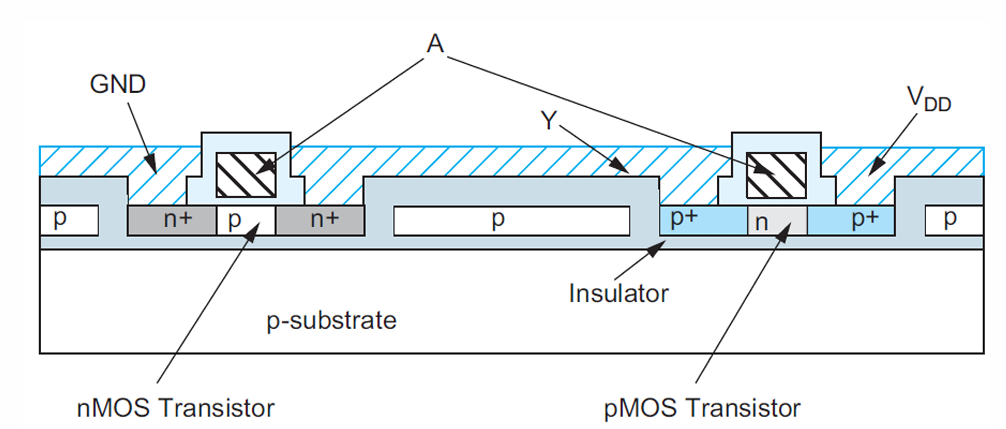
\includegraphics[width=\textwidth]{img/TX_img/soi.png}
        \caption{SOI}
        \label{}
    \end{subfigure}
    \hfill
    % --- Subfigure (b) ---
    \begin{subfigure}{0.5\linewidth}
        \centering
        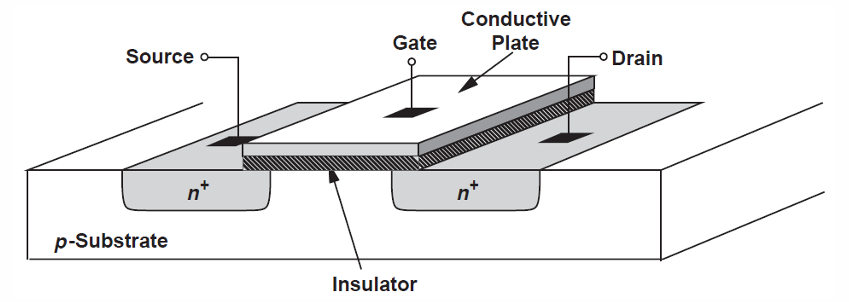
\includegraphics[width=\textwidth]{img/TX_img/bulk.png}
        \caption{Bulk MOSFET}
        \label{}
    \end{subfigure}
    \hfill
    \vspace{0.3cm}
    \caption{}
    \label{fig:NRZ SST}
\end{figure}
\section{Comparative Analysis: Regular Well vs. Flip-Well Architecture}

The 22nm FD-SOI technology offers two primary well configurations, each providing different biasing capabilities for N-FET and P-FET devices:

\subsection{Regular Well (Standard Well)}
In a standard configuration, transistors are placed over wells of the opposite doping type (N-FET in a P-well, P-FET in an N-well).
\begin{itemize}
    \item \textbf{Biasing Type}: Primarily optimized for \textbf{Reverse Body Biasing (RBB)}.
    \item \textbf{Operation}: Applying the lowest voltage to the P-well increases the threshold voltage ($V_{th}$), which significantly reduces leakage power at the cost of switching speed.
    \item \textbf{Use Case}: Ideal for low-power blocks where leakage reduction is more critical than high-speed performance.
\end{itemize}

\subsection{Flip-Well (Flipped-Well)}
In a Flip-Well architecture, the doping polarities of the underlying wells are reversed, placing transistors over wells of the same doping type (N-FET in an N-well, P-FET in a P-well).
\begin{itemize}
    \item \textbf{Forward Body Biasing (FBB)}: This configuration allows for aggressive Forward Body Biasing, often exceeding $2\,$V.
    \item \textbf{Performance Boost}: FBB significantly lowers the $V_{th}$ and increases the drive current ($I_{on}$), which is essential for reaching the high data rates required by the PCIe SERDES.
    \item \textbf{Tunability}: It enables a "tunable" transistor that can transition between high-performance modes and low-leakage idle states.
    
\end{itemize}

\begin{table}[htbp]
    \centering
    \caption{Strategic Differences Between Regular and Flip-Well FD-SOI}
    \label{tab:well_comparison}
    \begin{tabular}{l l l}
        \toprule
        \textbf{Feature} & \textbf{Regular Well} & \textbf{Flip-Well} \\
        \midrule
        N-FET Placement & P-well & N-well \\
        P-FET Placement & N-well & P-well \\
        Primary Bias Mode & Reverse Body Bias (RBB) & Forward Body Bias (FBB) \\
        Threshold Voltage ($V_{th}$) & Increased (High $V_{th}$) & Decreased (Low $V_{th}$) \\
        Leakage & Lowered & Significantly Increased \\
 
        \bottomrule
    \end{tabular}
\end{table}

\begin{figure}[H]
    \centering
    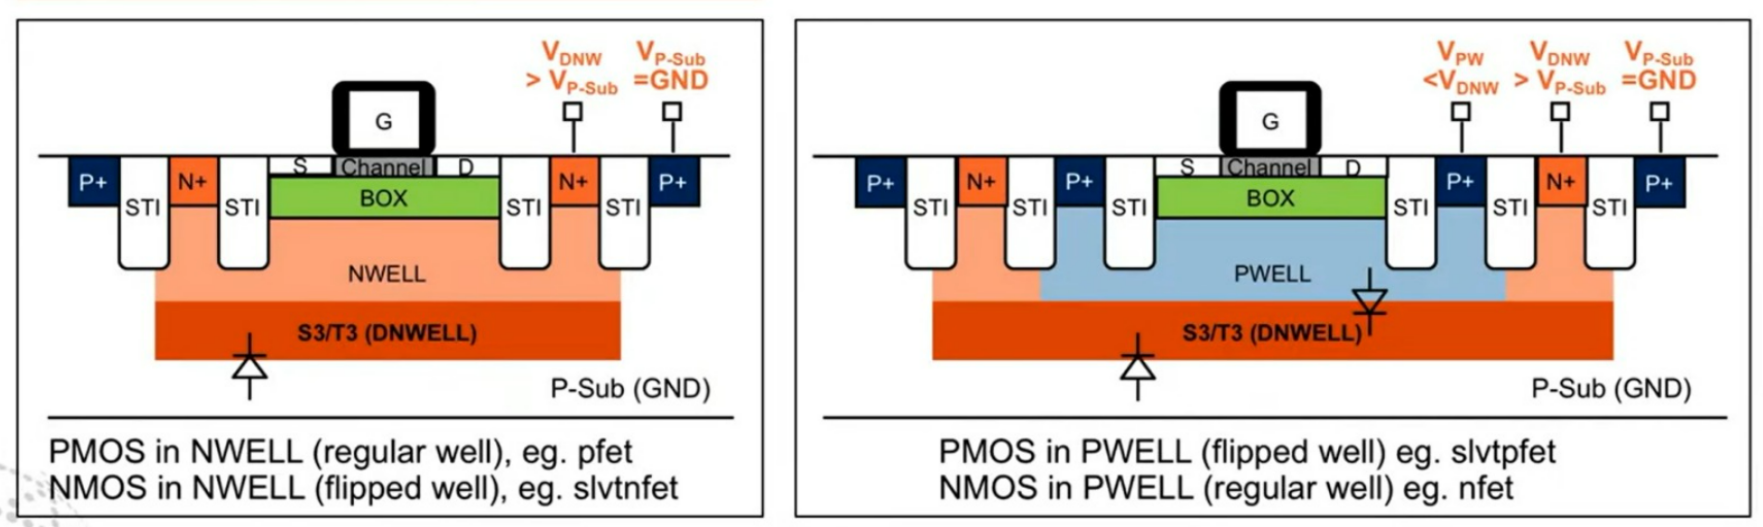
\includegraphics[width=1\textwidth]{img/TX_img/fwell.png}
    \caption{Structural illustration of Flip-Well vs. Conventional Well in FD-SOI.}
    \label{fig:flip_well}
\end{figure}





% ==================================================
% CHAPTER 2: FUNDAMENTALS & LIT REVIEW
% ==================================================
\chapter{System overview and Literature Architectures}
\label{ch:fundamentals}

\section{Clocking Systems in Wireline Transceivers}
\label{sec:clocking-systems}

In high-speed wireline communication, the clocking system is the "heartbeat" of the entire transceiver. Its primary function is to provide a precise time reference that dictates when data bits are generated, transmitted, and sampled. Without a highly stable clock, the synchronization between the transmitter (TX) Blocks would fail, leading to massive data corruption.

\subsection{The Role of Clocking in Serialization}
\label{subsec:role-clocking-serialization}

The most critical application of high-speed clocking within the transmitter is the \textbf{Serialization process}. In modern systems, data is processed internally in a parallel format (e.g., 32 or 64 bits wide) at a relatively low frequency to save power. To transmit this data over a single physical channel (like a copper trace or fiber), it must be converted into a serial bitstream.

The Serializer uses the clock signal to "multiplex" these parallel bits into a single high-speed line. For example, in a system aiming for a 64 Gbps data rate with 32Gbaud, the clocking network must provide timing edges that allow the serializer to place a new bit every \textbf{31.25 picoseconds}. Any misalignment or instability in this clock directly reduces the "eye opening" of the transmitted signal, making it harder for the receiver to distinguish between a digital '0' and '1'.

\begin{figure}[H]
    \centering
    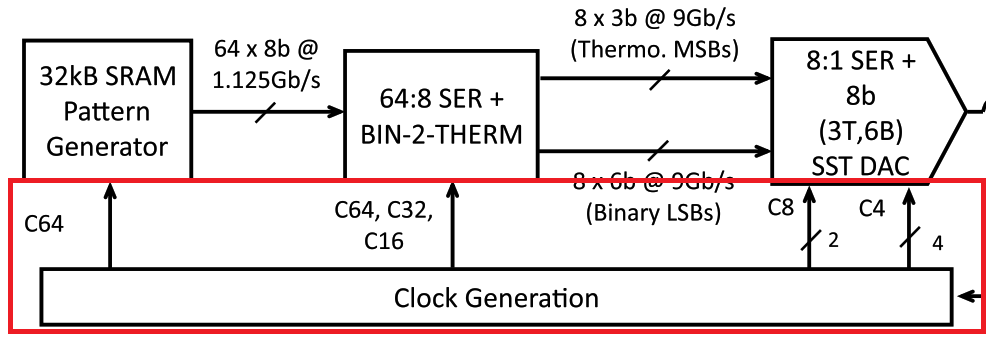
\includegraphics[width=0.8\textwidth]{img/TX_img/System.png}
    \caption{Clock Bundle in The System.}
    \label{fig:Wire Scaling}
\end{figure}

\section{Design Challenges in High-Frequency Clock Distribution}
\label{sec:design-challenges}

At a 32 GHz operating frequency, the clock period is \textbf{31.25 ps}. This extreme speed transforms the clock distribution network from a simple routing task into a complex high-frequency design problem. The challenges are primarily driven by the physical limitations of interconnects and the active circuitry required to drive them.

\subsection{Interconnect (Wire) Scaling and Bandwidth Limits}
\label{subsec:interconnect-scaling}

As CMOS technology scales to smaller nodes, the physical properties of on-chip metal wires become the dominant bottleneck.

\begin{itemize}
    \item \textbf{RC Delay and Scaling:} Every new technology node reduces the cross-sectional area of metal traces, which causes \textbf{Resistance (R)} to increase dramatically. Simultaneously, closer proximity to other wires increases parasitic \textbf{Capacitance (C)}. The resulting RC time constant of the wire limits how fast a signal can travel. At 32 GHz, even a relatively short wire can have a delay that is a significant fraction of the total clock period.
    
    \item \textbf{The RC-LPF Effect:} High-speed interconnects behave as a \textbf{Low-Pass Filter (LPF)}. This filter attenuates high-frequency components of the signal. Because a square-wave clock relies on high-frequency harmonics to maintain its shape, the wire "rounds off" the edges. By the time a 32 GHz signal travels across the transmitter, it loses its sharp transitions, making it difficult for the Serializer to detect valid clock edges.
\end{itemize}

\begin{figure}[H]
    \centering
    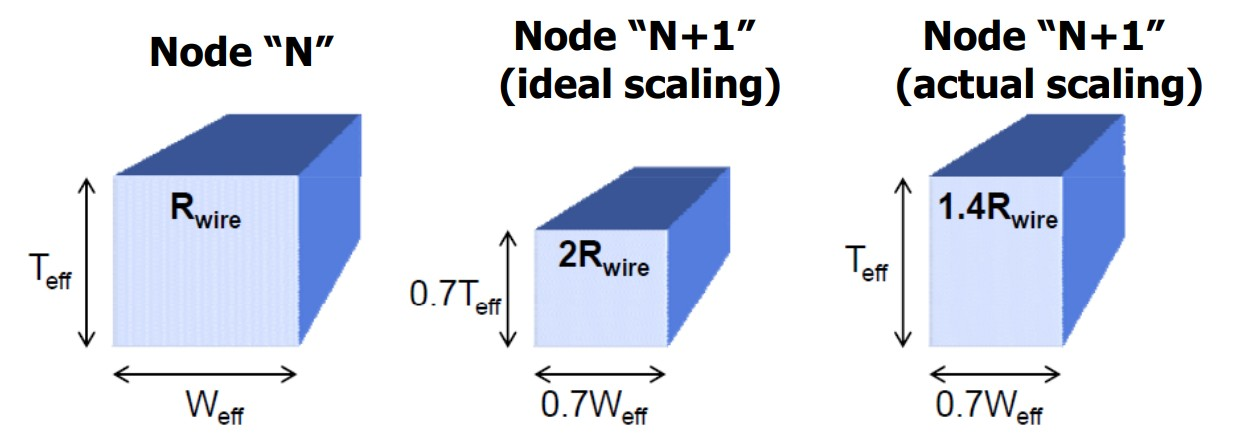
\includegraphics[width=0.7\textwidth]{img/TX_img/Wire_scaling.jpg}
    \caption{Impact of Technology Node Scaling on Wire Resistance and Geometry.}
    \label{fig:Wire Scaling}
\end{figure}


\subsection{Cascaded Clock Buffer Chains}
\label{subsec:cascaded-buffers}

Because the 32 GHz signal is severely attenuated by the\textbf{ LPF effect} and also increased delay due to wire resistance and the large capacitive load of the Serializer, it is physically impossible to drive the signal with a single buffer stage.

\begin{itemize}
    \item \textbf{The Repeater Strategy:} To maintain a usable voltage swing over the distance from the PLL to the Serializer, a chain of cascaded buffers must be placed along the path. These buffers act as "repeaters," re-amplifying the signal at regular intervals to combat the RC losses of the interconnects.
    
    \item \textbf{Load Management:} Each buffer must be sized to drive the input capacitance of the following stage. Since the GHz Serializer presents a massive capacitive load at an extremely high frequency, the final buffers in the chain must be exceptionally large. This results in significant power consumption and silicon area penalties.
\end{itemize}

\subsection{Jitter Amplification in Buffer Chains}
\label{subsec:jitter-amplification}

A major challenge with cascaded buffers at high frequencies is \textbf{Jitter Amplification}. This occurs when the clock frequency is close to the maximum bandwidth of the buffer.

\begin{itemize}
    \item \textbf{Limited Bandwidth Effect:} At 32 GHz, the clock period is so short (31.25 ps) that the transistors in the buffer may not have enough time to reach the full supply voltage (\(V_{DD}\)) or ground before the next transition begins. When the clock frequency operates close to the buffer's cutoff frequency, the buffer acts as a low-pass filter attenuating the signal and adds Jitter.
    
    \item \textbf{Noise-to-Jitter Conversion:} The limited bandwidth results in "rounded" edges with a slow \textbf{Slew Rate}. A slow slew rate is highly dangerous because it increases the \textbf{Rise} and \textbf{Fall} time of the signal. In this region, any small voltage noise (\(\Delta V\)) on the power supply or thermal noise from the transistors is translated into a large timing displacement (\(\Delta t\)), effectively "amplifying" the jitter.
    
    \item \textbf{Cumulative Degradation:} In a cascaded chain, each stage does not just pass the jitter of the previous stage; it adds its own noise and amplifies the existing timing uncertainty. By the time the 32 GHz clock reaches the Serializer, the accumulated jitter can consume a large portion of the Unit Interval (UI), leading to a significant increase in the Bit Error Rate (BER).
\end{itemize}

\begin{figure}[H]
    \centering
    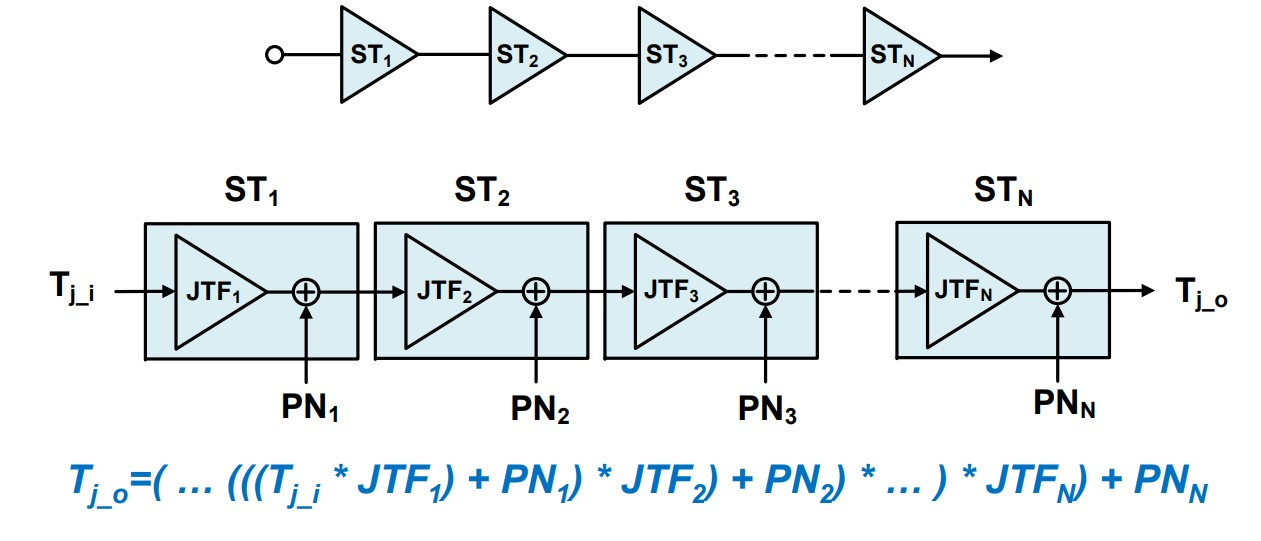
\includegraphics[width=0.8\textwidth]{img/TX_img/buffer_chain.jpg}
    \caption{Cumulative Jitter in Cascaded Clock Buffer Chains.}
    \label{fig:Wire Scaling}
\end{figure}

\subsection{Solution: Quadrature Clocking Scheme}
\label{sec:quadrature-solution}

To overcome the severe interconnect degradation and jitter amplification at High frequencies (eg. 32 GHz), modern high-speed transmitters utilize a \textbf{Quadrature Clocking Scheme}. This approach shifts the design strategy from "Brute Force" high-frequency distribution to a more efficient multi-phase architecture.

%\subsection{Frequency Reduction (Quarter-Rate Operation)}
%\label{subsec:frequency-reduction}
\begin{itemize}
    \item\textbf{Frequency Reduction (Quarter-Rate Operation):}

The most immediate benefit of the quadrature scheme is the reduction of the distribution frequency. By using four phases—\(0^\circ, 90^\circ, 180^\circ,\) and \(270^\circ\)—the system can operate at a "Quarter-Rate." which will effectively reduce \textbf {Power consumption} and \textbf{Jitter amplification}.

\begin{itemize}
    \item \textbf{Relaxed Bandwidth:} Instead of pushing a 32 $GHz$ signal through the buffer chains, the clocking blocks deliver an 8 GHz signal.
    
    \item \textbf{Combatting the RC-LPF:} At 8 GHz, the signal is much further away from the cutoff frequency of the on-chip interconnects. This results in significantly less amplitude attenuation and preserves the sharp edges of the clock, directly addressing the "Frequency Wall" mentioned in Section \ref{subsec:interconnect-scaling}.
\end{itemize}

\begin{figure}[H]
    \centering
    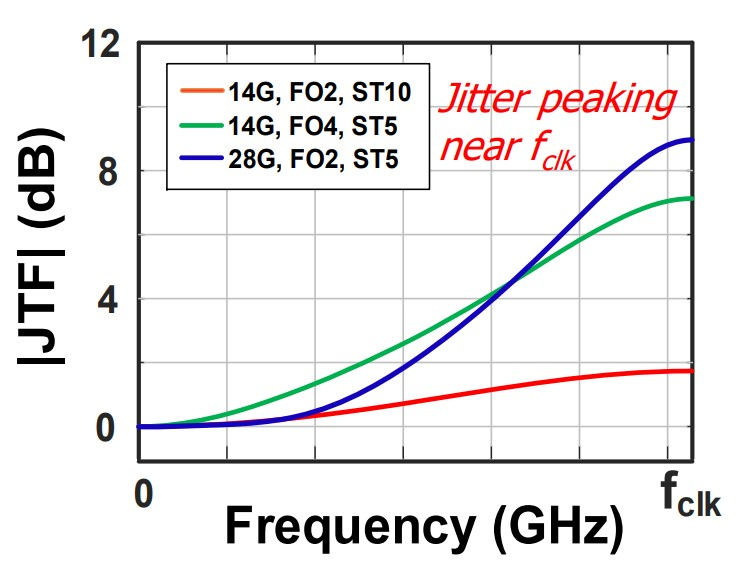
\includegraphics[width=0.8\textwidth]{img/TX_img/Jitter_amp.jpg}
    \caption{Jitter Transfer Function (JTF(dB)) vs. Clock Frequency.}
    \label{fig:Wire Scaling}
\end{figure}

\end{itemize}


%\subsection{Maintaining Data Throughput}
%\label{subsec:maintaining-throughput}
\begin{itemize}
    \item\textbf{Maintaining Data Throughput:}

The primary challenge in moving from a 32 GHz distribution to an 8 GHz distribution is maintaining the same data rate at the output The solution is not just using four phases, but specifically shaping those phases into a \textbf{25\% duty cycle}. This serves as the direct compensation for the slower clock speed.

\subsubsection{Replicating the 32 GHz Pulse Width}
In a full-rate 32 GHz system, each bit of data has a duration (Unit Interval or UI) of exactly 31.25 ps.

\begin{itemize}
    \item If we used a standard 8 GHz clock with a 50\% duty cycle, the "High" pulse would be \textbf{62.5 ps} long—twice as long as the required bit time.
    
    \item By enforcing a \textbf{25\% duty cycle} on the 8 GHz clock (\(125 \text{ ps} \times 0.25\)), we create a pulse that is exactly \textbf{31.25 ps} wide.
\end{itemize}

In this way, the 25\% duty cycle 8 GHz clock "mimics" the timing precision of the 32 GHz clock. It provides the exact same activation window for the serializer, but at a much lower repetition rate.

\subsubsection{Phase Interleaving for Full-Rate Throughput}
Because each 8 GHz phase now only occupies 25\% of the total cycle time, we can interleave four of these phases (\(0^\circ, 90^\circ, 180^\circ, 270^\circ\)) without any overlap.

\begin{itemize}
    \item Each phase is responsible for a different "time slot" in the 32 Gbps bitstream.
    
    \item As the first phase (\(0^\circ\)) finishes its 31.25 ps pulse, the second phase (\(90^\circ\)) immediately begins its 31.25 ps pulse.
\end{itemize}

This sequential "hand-off" between the four phases ensures that the Serializer is always active, producing a continuous stream of data at 32 Gbps. This effectively \textbf{compensates} for the 4\(\times\) reduction in frequency: the clock is 4\(\times\) slower, but because we use 4 phases with 1/4th the duty cycle, the data throughput remains identical to a 32 GHz system.

\subsubsection{Benefits of Compensation}
This compensation strategy allows the transmitter to enjoy the "best of both worlds":

\begin{enumerate}
    \item \textbf{Distribution Ease:} The wires and buffers only have to handle an 8 GHz fundamental frequency, avoiding the massive attenuation and quality loss of the 32 GHz "Frequency Wall" described in Section \ref{sec:design-challenges}.
    
    \item \textbf{Timing Accuracy:} The 25\% pulse width ensures the Serializer output maintains the correct bit period (\(31.25 \text{ ps}\)), preserving the "Data Eye" width for the receiver.
\end{enumerate}

\begin{figure}[H]
    \centering
    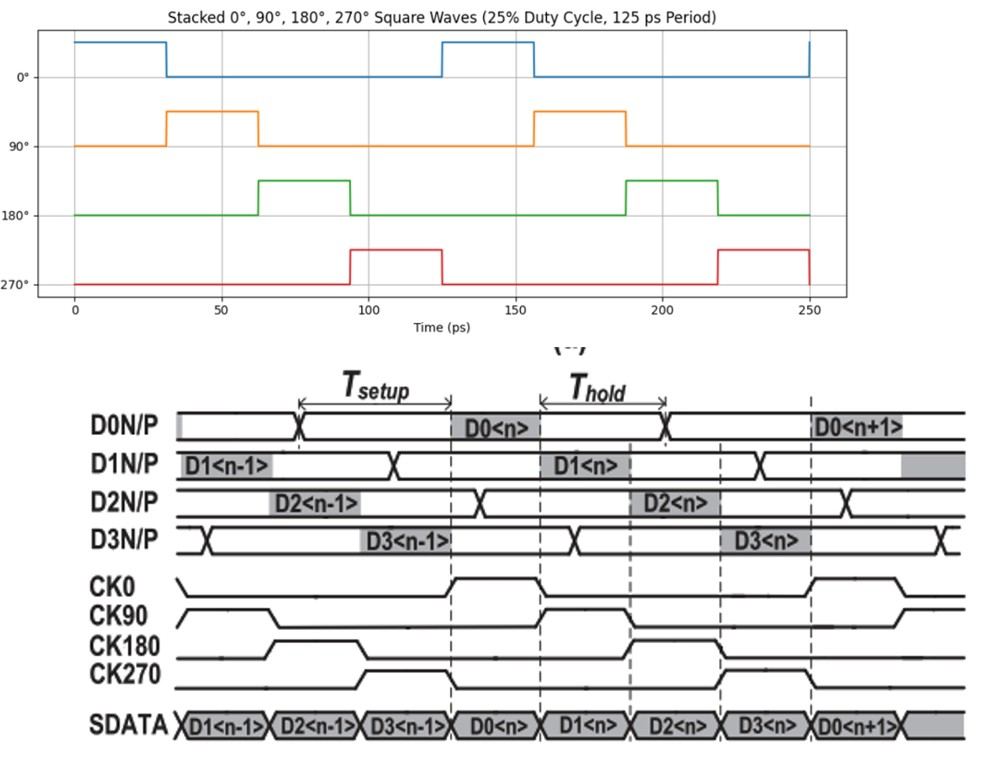
\includegraphics[width=0.8\textwidth]{img/TX_img/quarter_rate.jpg}
    \caption{Maintaining Data Throughput using Quarter Rate Clocking Scheme.}
    \label{fig:Wire Scaling}
\end{figure}

\end{itemize}

\section{Implementation Blocks for Quadrature Clocking}
\label{sec:implementation-blocks}

To implement a robust 8 GHz quadrature scheme, the transmitter clocking path integrates a series of specialized functional blocks. These blocks transform the raw high-frequency signal from the PLL into high-integrity timing pulses required by the Serializer.

\subsection{The I/Q Frequency Divider}
\label{subsec:iq-divider}

The I/Q Divider is the primary frequency translation element and the starting point of the local clock path.

\begin{itemize}
    \item \textbf{Function:} It receives the 32 GHz high-frequency reference from the PLL and divides it down to 8 GHz.
    
    \item \textbf{Quadrature Generation:} Utilizing a master-slave latch topology, it generates the four fundamental quadrature phases (\(0^\circ, 90^\circ, 180^\circ, 270^\circ\)) at a \textbf{50\% duty cycle}.
    
    \item \textbf{Challenges:} The divider must maintain high bandwidth to ensure that Division is done with low additional  jitter while operating at the limits of the technology node.
\end{itemize}

\subsection{Pulse Shaper (25\% Duty Cycle Generator)}
\label{subsec:pulse-shaper}

Since the I/Q divider produces 50\% duty cycle phases, a dedicated \textbf{Pulse Shaper} is required to prepare the clock for the quarter-rate serializer.

\begin{itemize}
    \item \textbf{Function:} This block performs a logic operation (typically an AND of overlapping quadrature phases) to reduce the pulse width from 50\% to \textbf{25\%}.
    
    \item \textbf{Frequency Compensation:} This creates the 31.25 ps window necessary to compensate for the reduced frequency, allowing the 8 GHz clock to drive a 32 Gbps bitstream with the same precision as a 32 GHz clock.
\end{itemize}

\subsection{Duty Cycle Correction (DCC) Circuits}
\label{subsec:dcc-circuits}

The DCC is a critical calibration block that maintains the integrity of the pulse width against PVT (Process, Voltage, Temperature) variations.

\begin{itemize}
    \item \textbf{50\% Correction Mode:} The DCC first ensures that the divider's outputs are perfectly symmetrical. If the 50\% duty cycle is distorted, it creates an immediate phase-shift error between the \(I\) and \(Q\) signals.
    
    \item \textbf{25\% Correction Mode:} The DCC also monitors the output of the Pulse Shaper. Because a 25\% pulse at 8 GHz is extremely narrow (31.25 ps), any drift can cause bit-width mismatch or data collisions in the Serializer. The DCC applies a correction voltage to "lock" the pulse width at exactly \(1/4\) of the clock period.
\end{itemize}

\subsection{Deskew Circuits}
\label{subsec:deskew-circuits}

The final block in the chain is the \textbf{Deskew} circuit, which provides the final "fine-tuning" of the timing edges.

\begin{itemize}
    \item \textbf{Function:} It provides independent delay control for each of the four quadrature phases.
    
    \item \textbf{Phase Orthogonality:} Even with a perfect divider, the physical metal routing to the Serializer can introduce "skew" (timing mismatches). Deskew circuits—usually digitally controlled delay lines—adjust the arrival of each phase to ensure they remain exactly \(90^\circ\) apart at the point of serialization.
    
    \item \textbf{System Impact:} This maximizes the horizontal timing margin (the "eye width") of the transmitted signal.
\end{itemize}

\subsection{Summary of Service}
\label{subsec:summary-service}

The I/Q Divider provides the raw phases, but open-loop division is susceptible to PVT (Process, Voltage, Temperature) variations. By including \textbf{DCC and Deskew circuits}, we create a robust clocking path that can calibrate itself to maintain 90\(^\circ\) precision and 50\% duty cycle regardless of manufacturing mismatches. This directly leads to a wider 'Data Eye' and a lower Bit Error Rate (BER) at the transmitter output.


\begin{table}[ht]
    \centering
    \caption{Quadrature Clocking Path Functional Blocks Summary}
    \label{tab:clocking-blocks}
    \begin{adjustbox}{width=\textwidth}
    \begin{tabular}{lcccc}
        \toprule
        \textbf{Block} & \textbf{Input Frequency} & \textbf{Output Frequency} & \textbf{Duty Cycle Focus} & \textbf{Primary Purpose} \\
        \midrule
        \textbf{I/Q Divider} & 16 GHz & \textbf{8 GHz} & 50\% & Frequency reduction \& \(I/Q\) generation \\
        \textbf{Pulse Shaper} & 8 GHz & \textbf{8 GHz} & 25\% & Frequency compensation (31.25 ps pulse) \\
        \textbf{DCC} & 8 \GHz & \textbf{8 \GHz} & 50\% \& 25\% & Preventing Duty Cycle Distortion (\DCD) \\
        \textbf{Deskew} & 8 \GHz & \textbf{8 \GHz} & Phase Alignment & Correcting routing-induced phase skew \\
        \bottomrule
    \end{tabular}
    \end{adjustbox}
\end{table}

\section{Jitter in High-Speed Clocking}
\label{sec:jitter-analysis}

Following the hardware implementation, it is essential to analyze the timing uncertainty, or jitter, that these blocks introduce. At 32 Gbps, jitter management is the primary factor in determining the system's reliability.

\subsection{Eye Diagram and Specification Mask}
\label{subsec:eye-diagram}

For proper operation, high-speed links must maintain margin in both the voltage and timing domains.

\begin{itemize}
    \item \textbf{Interoperability:} To allow independent design of the transmitter (TX) and receiver (RX), a "spec eye mask" is used, which is determined by the specific industry standard (e.g., PCIe, Ethernet).
    
    \item \textbf{Performance Guarantee:} The signal must not violate this mask to guarantee a minimum level of performance.
\end{itemize}

\begin{figure}[H]
    \centering
    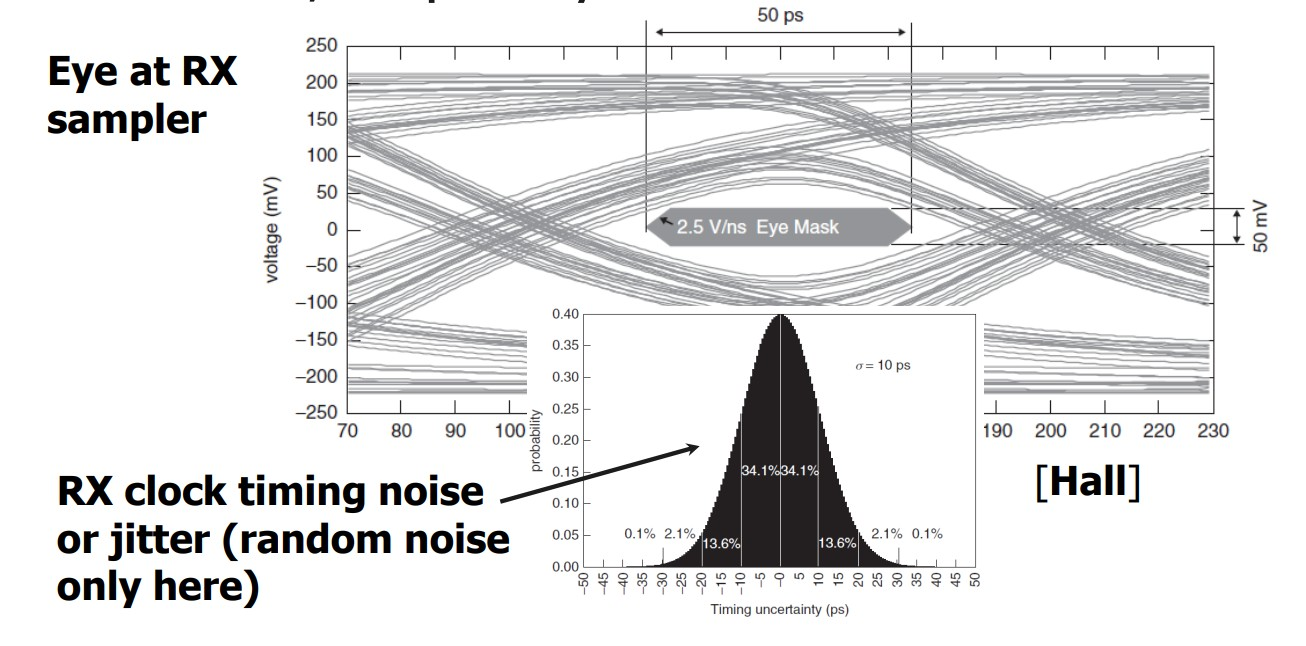
\includegraphics[width=0.8\textwidth]{img/TX_img/Eye_mask.jpg}
    \caption{Spec Mask.}
    \label{fig:Wire Scaling}
\end{figure}


\subsection{Jitter Definitions and Measurements}
\label{subsec:jitter-definitions}

Based on how we observe the signal, jitter is categorized into three measurement types:

\begin{itemize}
    \item \textbf{Period Jitter (\(J_{\text{PER}}\)):} The deviation of a single clock period from the ideal period (\(T_{\text{ideal}}\)). It is the most basic measure of clock stability.
    
    \item \textbf{Cycle-to-Cycle Jitter (\(J_{\text{CC}}\)):} The difference in duration between two consecutive clock periods. Important for budgeting on-chip digital circuits cycle time.
    
    \item \textbf{Accumulated Jitter (\(J_{\text{AC}}\)):} Also known as Long-Term Jitter, it measures the displacement of a clock edge relative to an ideal trigger after \(N\) cycles. This is the most critical metric for our transmitter, as it defines how much the clock drifts over the time required for serialization.
\end{itemize}

\begin{figure}[H]
    \centering
    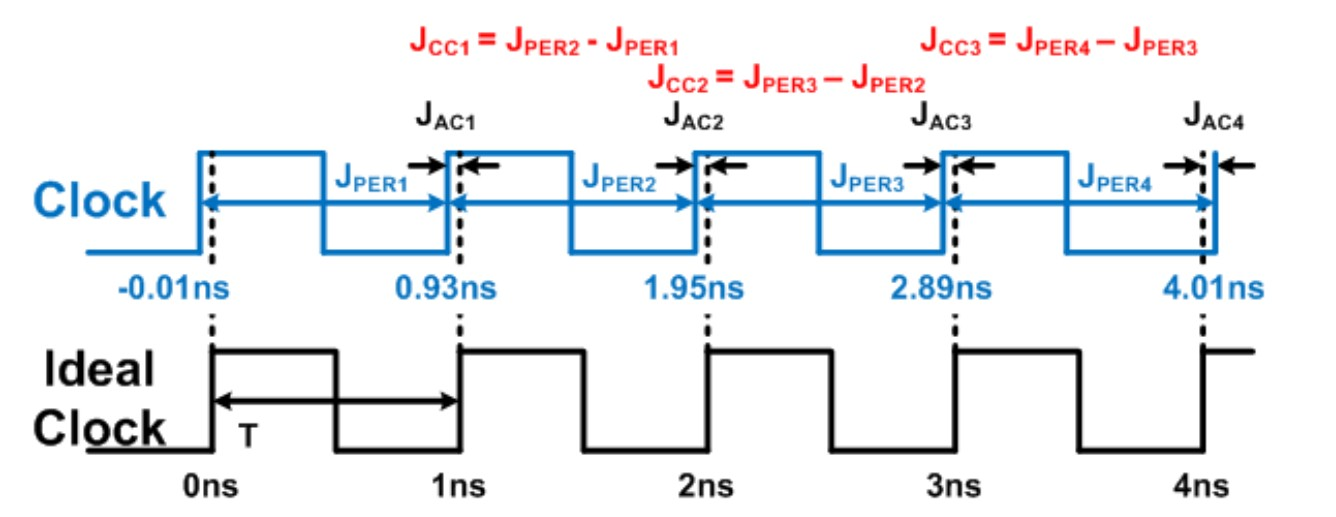
\includegraphics[width=0.8\textwidth]{img/TX_img/jitter_param.jpg}
    \caption{Jitter Definitions.}
    \label{fig:Wire Scaling}
\end{figure}

\subsection{Jitter Statistical Parameters}
\label{subsec:statistical-parameters}

Since jitter is a stochastic (random) process, we describe it using statistical metrics:

\begin{itemize}

\item \textbf{Mean Value:}
    Can be interpreted as a fixed timing offset or “skew”, Generally not important, as usually can corrected for.



    \item \textbf{RMS Jitter (\(\sigma\)):} The standard deviation of the jitter distribution. It is used to describe Random Jitter (\(\RJ\)).
    
    \item \textbf{Peak-to-Peak Jitter (\(J_{\text{PP}}\)):} Function of both deterministic (bounded) and random
    (unbounded) jitter components, Must be quoted at a given BER to account for random
    (unbounded) jitter.
    
\end{itemize}

\subsection{Detailed Classification of Jitter Components}
\label{subsec:jitter-classification}

Total Jitter (\(\TJ\)) is the result of various independent, correlated and uncorrelated noise sources. To manage a 64 Gbps link, we must categorize these components based on their statistical properties.

\subsubsection{Random Jitter (\(\RJ\))}
Random Jitter is timing noise that is unpredictable and follows a stochastic process.

\begin{itemize}
    \item \textbf{Sources \& Causes:}
    \begin{itemize}
        \item \textbf{Thermal Noise:} Generated by the random motion of electrons in conductors and transistors. It increases with temperature.
        \item \textbf{Flicker Noise (\(1/f\)):} Low-frequency noise caused by "traps" at the silicon-dielectric interface.
    \end{itemize}
    
    \item \textbf{Characteristics:}
    \begin{itemize}
        \item\ \textbf{unbounded}, follows a \textbf{Gaussian (Normal) Distribution} 
        \item\ Assumed to have zero mean value.
        \item\  It is quantified by its RMS value (\(\sigma\)).
    \end{itemize}
\end{itemize}

\begin{equation}
    \centering
    RJ(t) = \frac{1}{\sqrt{2\pi}\sigma_{RJ}} e^{\frac{-t^2}{2\sigma_{RJ}^2}}
\end{equation}

\begin{figure}[H]
    \centering
    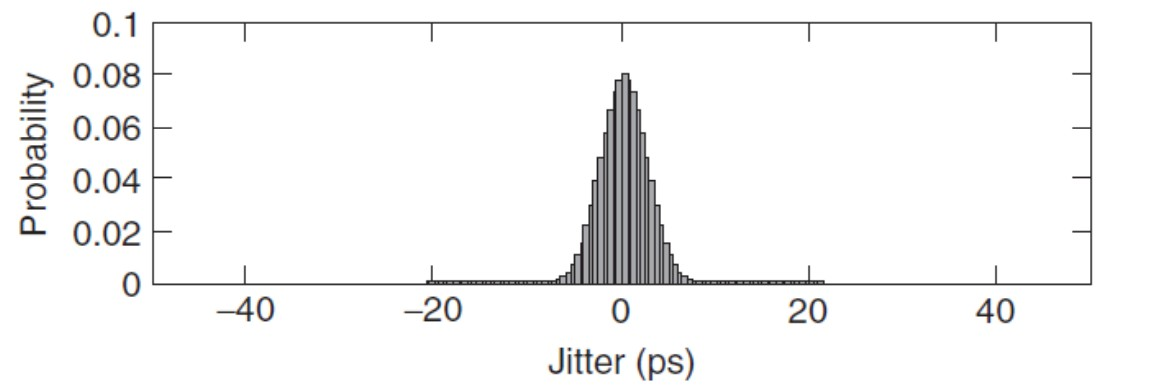
\includegraphics[width=0.8\textwidth]{img/TX_img/RJ.jpg}
    \caption{Probability Density Function (PDF) of Random Jitter.}
    \label{fig:Wire Scaling}
\end{figure}

\subsubsection{Deterministic Jitter (\(\DJ\))}
Deterministic Jitter is bounded; it has a specific maximum peak-to-peak value.
\begin{itemize}
    \item \textbf{causes:}
    \begin{itemize}
    \item \ Transmission-line losses (ISI)
    \item\ Duty Cycle Distortion (DCD)
    \item\ Spread Spectrum Clocking
    \item\ Crosstalk
    \end{itemize}
\end{itemize}

\begin{figure}[H]
    \centering
    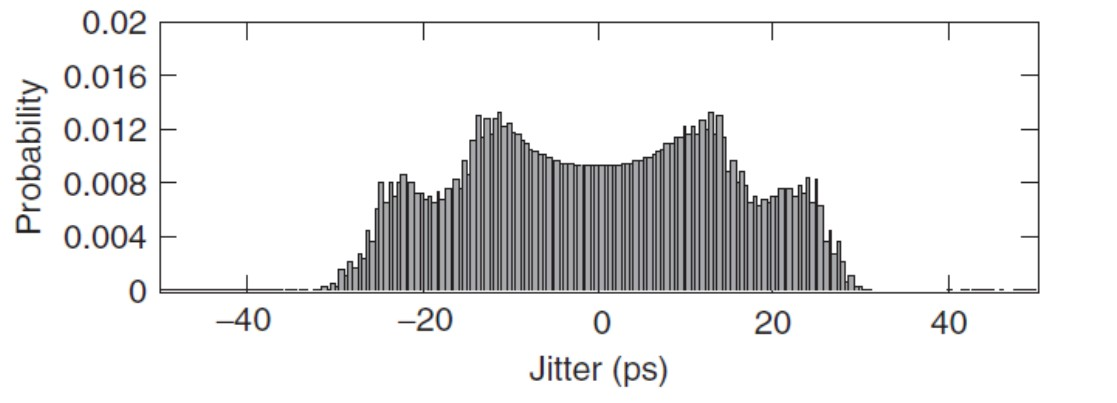
\includegraphics[width=0.8\textwidth]{img/TX_img/DJ.jpg}
    \caption{Probability Density Function (PDF) of Determinstic Jitter.}
    \label{fig:Wire Scaling}
\end{figure}

\subsubsection{Sinusoidal or Periodic Jitter (SJ or PJ):} 
Repeats at a fixed frequency due to modulating effects.

\begin{itemize}
    \item \textbf{Spread spectrum clocking:}
    \item \textbf{PLL reference clock feedthrough:}
\end{itemize}

\begin{equation}
    \centering
    PDF_{SJ}(t) = 
    \begin{cases} 
      \frac{1}{\pi\sqrt{A^2 - t^2}} & A > |t| \\
      0 & A \leq |t| 
    \end{cases}
\end{equation}

\begin{figure}[H]
    \centering
    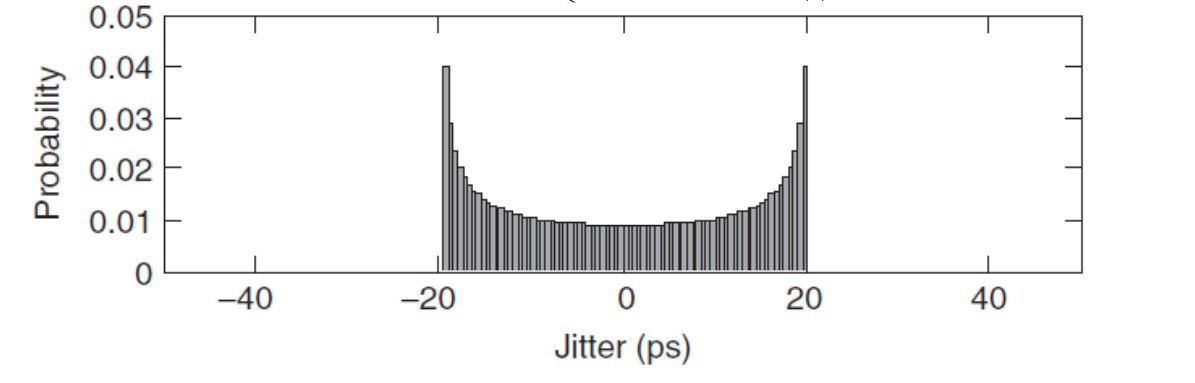
\includegraphics[width=0.8\textwidth]{img/TX_img/SJ.jpg}
    \caption{Probability Desity Function (PDF) of Sinusoidal Jitter.}
    \label{fig:Wire Scaling}
\end{figure}

\subsubsection{Data-Dependent Jitter (DDJ):}
    Data dependent jitter is correlated with either the transmitted data pattern or aggressor (crosstalk).

\begin{itemize}
    \item \textbf{Intersymbol Interference (ISI):}
    \begin{itemize}
        \item \textbf{Source:} Caused by channel loss, dispersion, and reflections.
        \item \textbf{Cause:} As discussed in the 32 GHz challenges, the RC-LPF effect prevents the signal from reaching full rail-to-rail swing before the next transition. The "memory" of previous bits shifts the threshold crossing point of the current bit.
        \item Can be improved by equalitzation.

\begin{figure}[H]
    \centering
    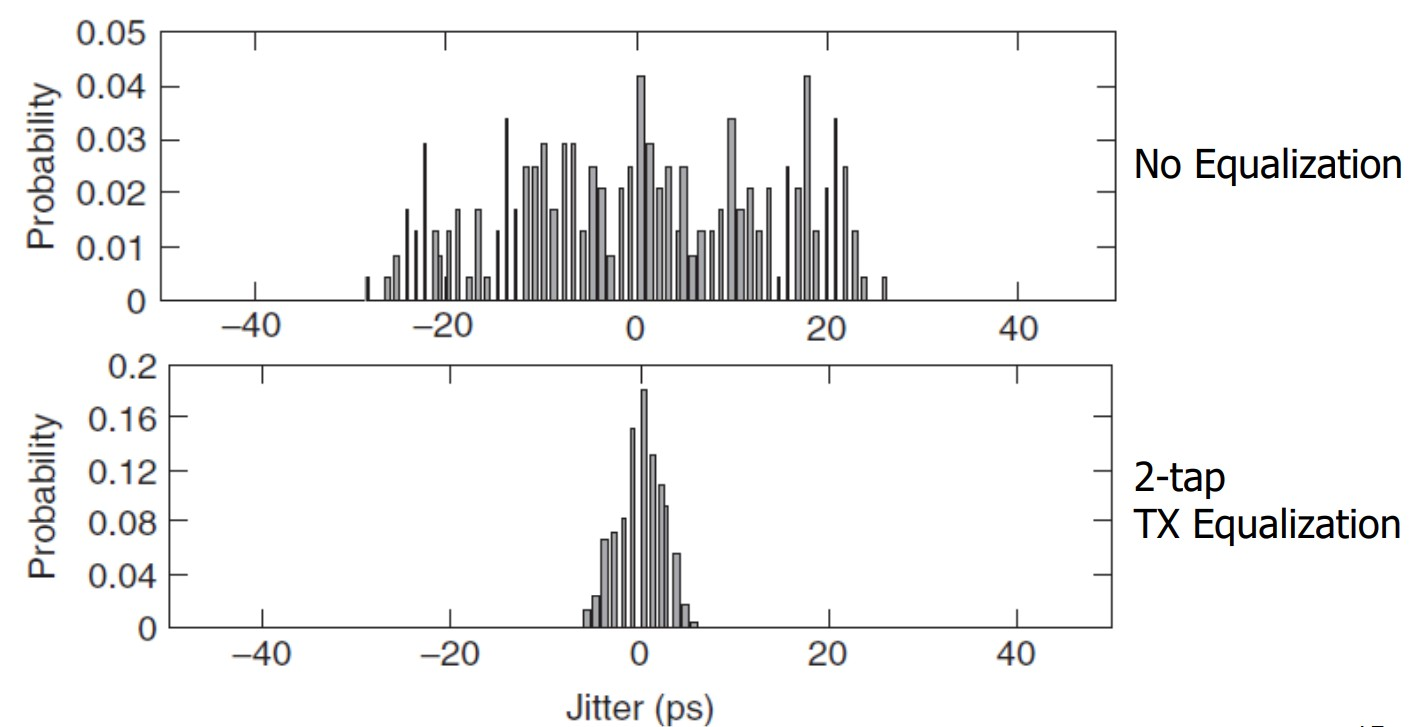
\includegraphics[width=0.8\textwidth]{img/TX_img/ISI.jpg}
    \caption{Probability Density Function (PDF) Of Inter-Symbol Interference Jitter.}
    \label{fig:Wire Scaling}
\end{figure}
        
    \end{itemize}
\end{itemize}

\begin{itemize}
    \item \textbf{Duty Cycle Distortion (DCD):}
    \begin{itemize}
        \item \textbf{Source:} Caused by duty cycle errors in TX serialization clocks and rise/fall delay mismatches.
        \end{itemize}
       \begin{itemize}
        \item \textbf{Rise/Fall Time Mismatch:} The buffers driving the output often have different slew rates for rising and falling edges. This is primarily caused by unequal strengths (W/L ratios) or switching speeds between PMOS and NMOS transistors.
        \item \textbf{Voltage Offsets:} DC offsets in the differential signals of the I/Q divider, often due to process variations or threshold voltage (\(V_{\text{th}}\)) mismatches, cause the signal to cross the switching threshold earlier or later than intended.
    \end{itemize}
    \item \textbf{Effect:}
    \begin{itemize}
        \item \textbf{Window Shrinkage:} DCD deviates the clock from the ideal 50\% or 25\% duty cycle. This results in the "sampling" windows for the four quadrature phases being unequal in width.
        \item \textbf{Bit-Width Mismatch:} One bit in the 32 Gbps stream becomes wider while the next becomes narrower. This "non-ideal zero-crossing" reduces the horizontal timing margin (eye-width), making the system highly sensitive to error at the Serializer output.
    \end{itemize}
\end{itemize}


\begin{equation}
    \centering
    PDF_{DCD}(t) = \frac{1}{2} \left[ \delta\left(t - \frac{\alpha_{DCD}}{2}\right) + \delta\left(t + \frac{\alpha_{DCD}}{2}\right) \right]
\end{equation}

\begin{figure}[H]
    \centering
    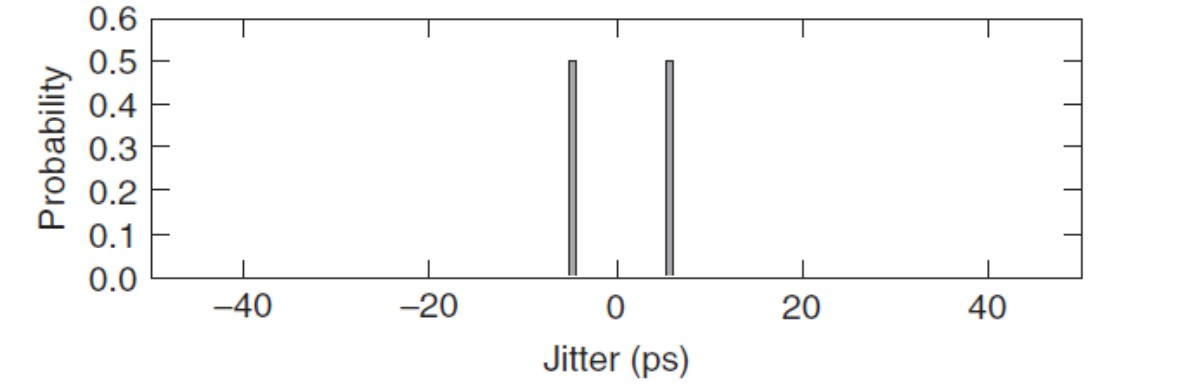
\includegraphics[width=0.8\textwidth]{img/TX_img/DCD.jpg}
    \caption{Probability Desity Function (PDF) of Duty Cycle Distortion Jitter.}
    \label{fig:Wire Scaling}
\end{figure}


\begin{itemize}
\item \textbf{Bounded Uncorrelated Jitter (BUJ):}


\begin{itemize}
    \item \textbf{Source:} Primarily \textbf{Crosstalk}.
    \item \textbf{Cause:} When a nearby high-speed signal (aggressor) switches, it injects a current spike into the clock line (victim) via mutual capacitance or inductance.
    \item \textbf{Characteristics:} It is "Uncorrelated" because the aggressor's data usually has no relationship with the clock, but it is "Bounded" because the interference has a maximum physical limit.
    \end{itemize}
\end{itemize}


\subsection{Total Jitter (TJ)}
The total jitter PDF is produced by convolving the random and deterministic jitter PDFs.
The Total Jitter (TJ) represents the overall timing uncertainty in the system. The probability density function (PDF) of total jitter is mathematically derived by convolving the individual PDFs of random and deterministic jitter components:

\begin{equation}
    PDF_{JT}(t) = PDF_{RJ}(t) * PDF_{DJ}(t)
\end{equation}

where the deterministic jitter PDF is itself a result of the convolution of several sub-components, including Periodic (Sinusoidal) Jitter ($SJ$), Duty Cycle Distortion ($DCD$), Intersymbol Interference ($ISI$), and Bounded Uncorrelated Jitter ($BUJ$):

\begin{equation}
    PDF_{DJ}(t) = PDF_{SJ}(t) * PDF_{DCD}(t) * PDF_{ISI}(t) * PDF_{BUJ}(t)
\end{equation}

\begin{figure}[H]
    \centering
    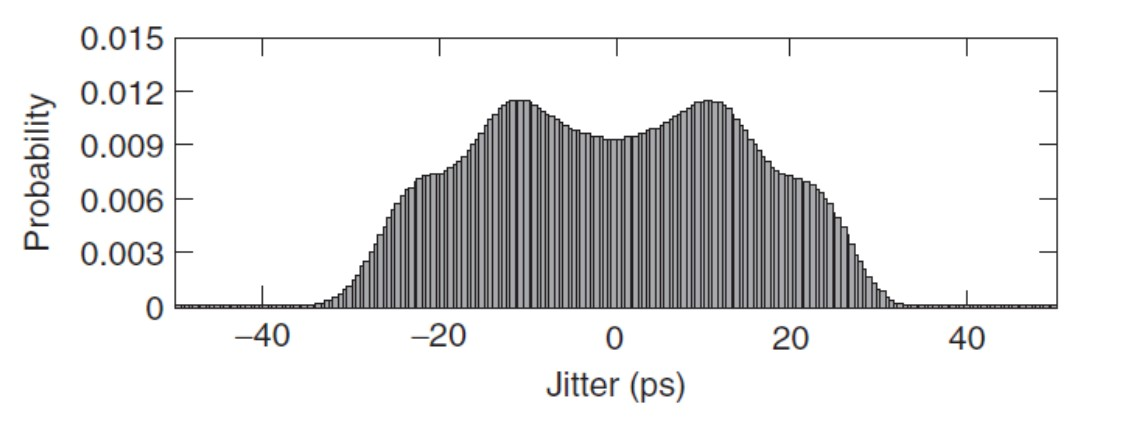
\includegraphics[width=0.8\textwidth]{img/TX_img/TJ.jpg}
    \caption{Probability Desnity Function (PDF) of Total Jitter .}
    \label{fig:Wire Scaling}
\end{figure}


\subsection{System Jitter Budgeting}
\label{subsec:jitter-budgeting}

Jitter budgeting is the mathematical process used to ensure that the cumulative timing uncertainty from all sources—transmitter, clock distribution, and channel—does not exceed the Unit Interval (UI). To guarantee a specific Bit Error Rate (BER), jitter components must be combined according to their statistical nature.

\subsubsection{Linear Addition of Deterministic Jitter (\(\DJ\))}
Deterministic Jitter components are bounded and have fixed peak-to-peak values. The convolution of multiple bounded jitter distributions is approximated by the linear sum of their individual peak-to-peak terms:

\begin{equation}
    D_{J,\text{total}} = \sum D_{J,i} = D_{J,\text{ISI}} + D_{J,\text{DCD}} + D_{J,\text{Pj}} + \cdots
\end{equation}

Since \(\DJ\) is not random, every pico second of deterministic jitter added to the system directly reduces the available timing window for sampling.

\subsubsection{Root-Sum-Square (RSS) of Random Jitter (\(\RJ\))}
Random jitter sources (such as thermal and shot noise) are uncorrelated and follow a Gaussian distribution. To calculate the total system \(\RJ\), the RMS values are combined using the RSS method:

\begin{equation}
    \sigma_{\RJ,\text{total}} = \sqrt{\sigma_{\RJ,1}^2 + \sigma_{\RJ,2}^2 + \sigma_{\RJ,3}^2 + \cdots}
\end{equation}

This statistical approach is used because it is highly improbable for multiple independent random noise sources to reach their peak displacement simultaneously.

\subsubsection{Total Jitter (TJ) and the Dual-Dirac Model}
The Dual-Dirac model is the industry standard for predicting eye closure at a specific BER. It combines the bounded \(\DJ\) and the unbounded Gaussian \(\RJ\):

\begin{equation}
    T_J(\text{BER}) = D_{J,pp} + Q(\text{BER}) \cdot \sigma_{R_J,total}
\end{equation}

\begin{itemize}
    \item \textbf{The Q-Factor:} This multiplier represents the number of standard deviations required to achieve a target probability on the Gaussian tails.
    
    \item \textbf{The \(14\sigma\) Rule:} For a common target of BER = \(10^{-12}\), the \(Q\) factor is approximately 14 (representing \(7\sigma\) on each side of the transition). In this case, the equation becomes:
    \end{itemize}
    
   \begin{equation}
    T_J = D_{J,pp} + 14 \cdot \sigma_{R_J,total}
\end{equation}

\subsubsection{The Timing Margin Requirement}
A high-speed link is considered functional only if the Total Jitter is less than the Unit Interval, leaving sufficient margin for the receiver:

\begin{equation}
    \UI \geq \TJ(\BER) + \text{Receiver Margin}
\end{equation}

If the total jitter exceeds the UI, the "Data Eye" closes, and the receiver will be unable to distinguish between bit transitions, leading to a failure to meet the BER target. Design techniques such as Duty Cycle Correction (DCC) and Deskewing are employed specifically to reclaim this timing margin by minimizing the \(\DJ\) components.

\begin{figure}[H]
    \centering
    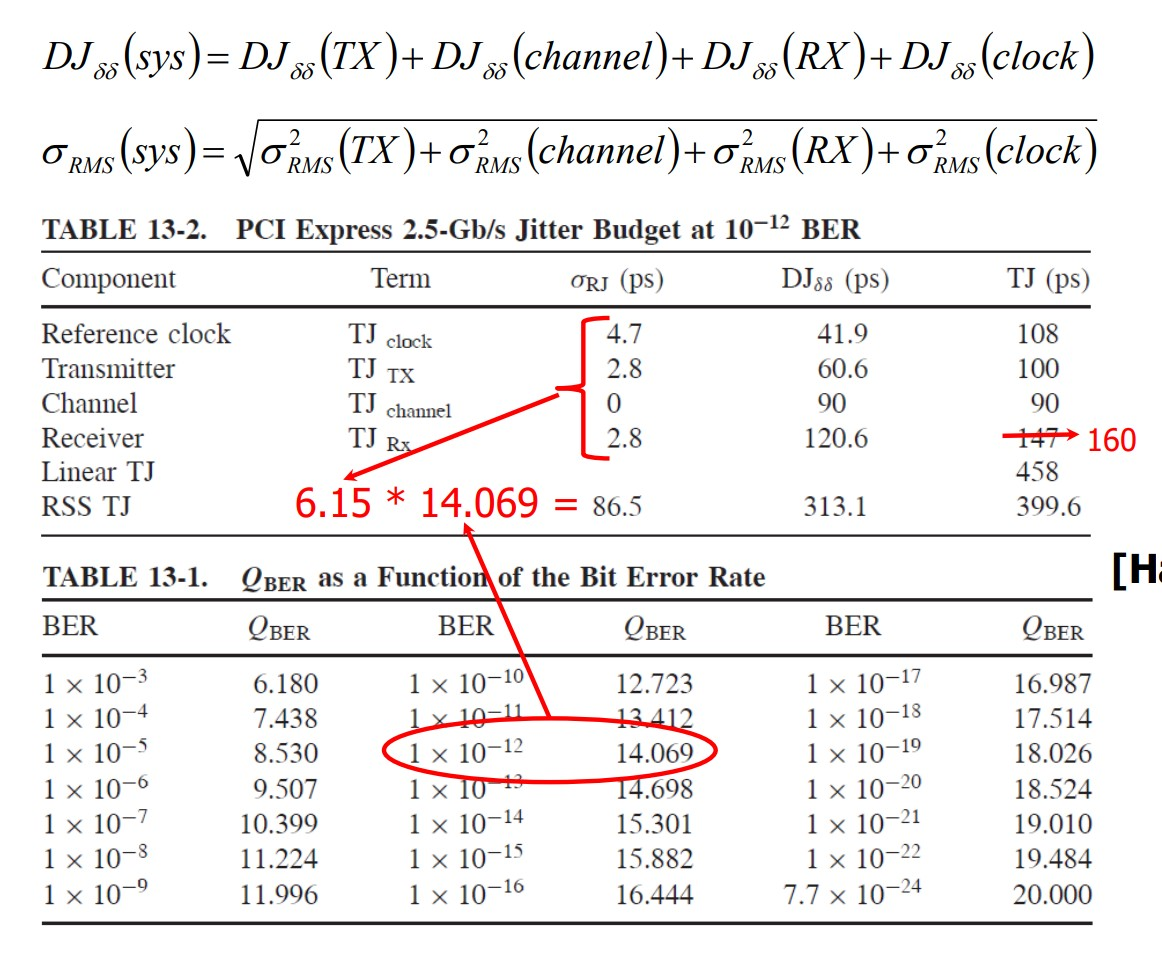
\includegraphics[width=0.8\textwidth]{img/TX_img/Jitter_ex.jpg}
    \caption{Jitter budgeting Example.}
    \label{fig:Wire Scaling}
\end{figure}


% ==================================================
% CHAPTER 1: INTRODUCTION
% ==================================================
\setcounter{page}{1}   % Reset counter to 1 for the Introduction
\section{Fundamentals of High-Speed Serialization}
The core function of a high-speed transmitter is to convert parallel low-speed data from the digital core into a serial high-speed stream suitable for transmission over the physical medium. This Parallel-In Serial-Out (PISO) operation is the final and most critical stage of the digital-to-analog interface. As data rates scale towards 64 Gb/s and beyond, the serializer (Multiplexer or Mux) becomes the primary bandwidth bottleneck. This chapter reviews the fundamental serialization architectures and presents a literature survey of circuit topologies used to implement the high-speed multiplexer.

\subsection{The Parallel-In Serial-Out (PISO) Concept}
A PISO block receives $N$ parallel data streams, each running at a frequency of $f_{clk}/N$, and interleaves them into a single serial stream running at the full baud rate $f_{baud}$. In the context of PAM4 signaling, the serializer operates on symbols rather than individual bits. For a 64 Gb/s PAM4 link, the symbol rate is 32 Gbaud.

The design of the PISO stage is governed by the trade-off between the complexity of the clock distribution network and the switching speed of the multiplexing circuits.

\begin{figure}[H]
    \centering
    % REPLACE 'piso.jpg' with your filename
    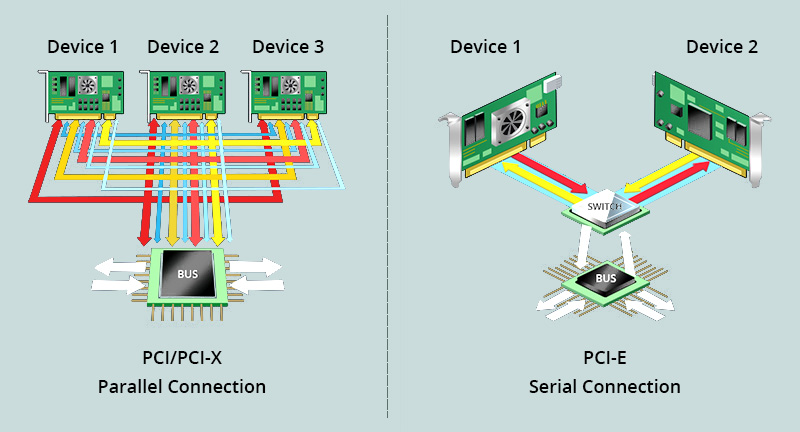
\includegraphics[width=0.8\textwidth]{img/TX_img/piso.jpg}
    \caption{Conceptual operation of the Parallel-In Serial-Out (PISO) block: Converting parallel low-speed data streams into a single high-speed serial output.}
    \label{fig:piso_diagram}
\end{figure}
\clearpage
\subsection{System-Level Placement of the : 4:1 High-Speed Multiplexer and Pre-Driver}
\label{subsec:system_level_placement_mux}

The high-speed multiplexer (MUX) and integrated pre-driver chain serve as the final digital stage within the transmitter serialization architecture. Positioned at the very end of the digital serialization domain, this integrated macro links the low-speed digital core with the high-speed analog front-end macros. 

\subsubsection{Data Path Context and Interface Boundaries}

The data path position of this macro is defined by its incoming and outgoing interface parameters:
\begin{itemize}
    \item \textbf{Input Interface:} The block receives 4 parallel lanes from the upstream digital serialization core (post-64:4 digital core serialization) with an input symbol period of $125\text{ ps}$.
    \item \textbf{Output Interface:} The core multiplexer logic merges these parallel streams into a single serial stream, which is delivered directly to the analog output stage with a compressed symbol period of $31.25\text{ ps}$.
\end{itemize}

\begin{figure}[H]
    \centering
    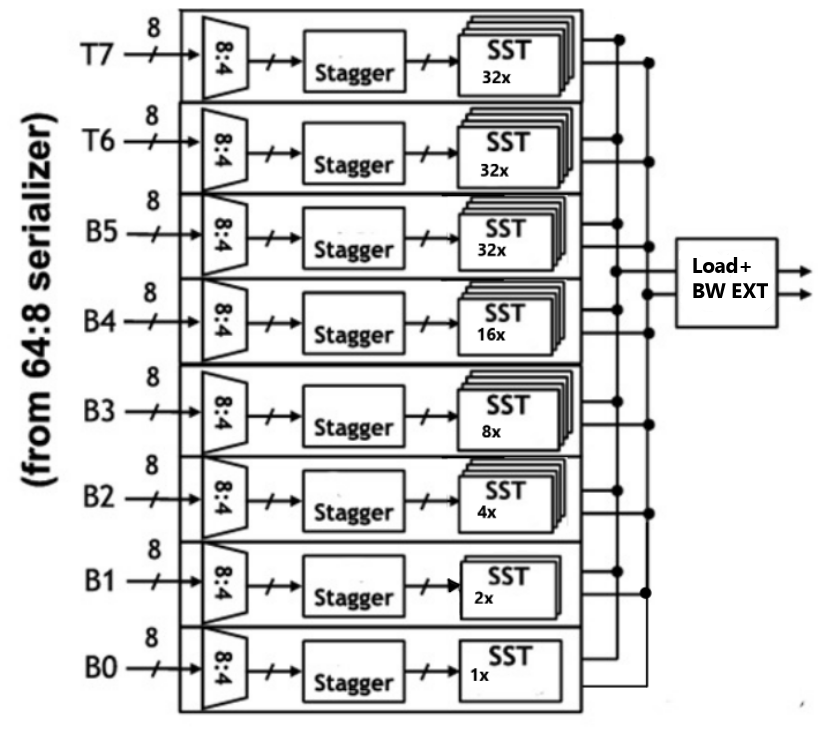
\includegraphics[width=0.9\textwidth]{img/TX_img/dac_based_architecture.png}
    \vspace{1mm} 
    \caption{Architectural overview of the DAC-Based Transmitter.}
    \label{fig:transmitter_macro_overview}
\end{figure}

\subsubsection{Timing Constraints}

Because the output data tracks run with a symbol period of $31.25\text{ ps}$, this integrated block is the fastest digital section in the entire transmitter macro. The physical routing channels and stage transitions must handle picosecond-level timing budgets to preserve the integrity of the data stream. 

To satisfy these tight timing constraints, the staggered 4-bit parallel data ($D4\langle0:3\rangle$) is fed into a high-speed 4:1 multiplexer core before driving the active pre-driver staging, which provides the necessary signal sharpening to drive the final source-series terminated (SST) analog driver stage.

\begin{figure}[H]
    \centering
    % Place holder for the 4:1 MUX -> Pre -> SST block slice diagram
     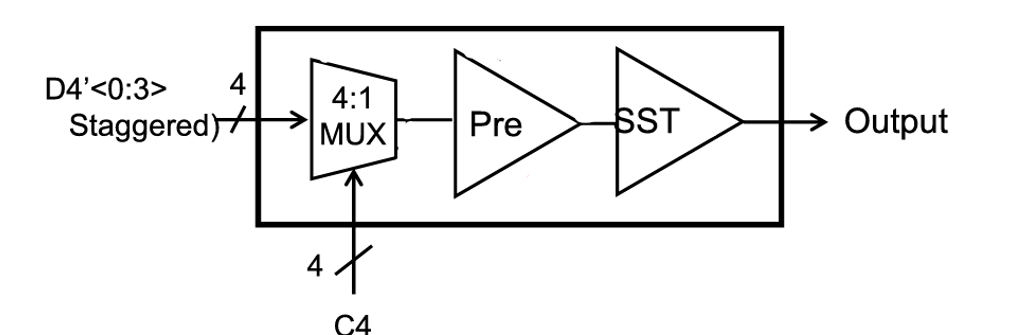
\includegraphics[width=0.75\textwidth]{img/TX_img/mux_predriver_sst_slice.png}
    \vspace{1mm} 
    \caption{Detailed schematic slice of the standalone serialization branch showing the 4:1 multiplexer cell, active pre-driver buffers, and the analog output driver.}
    \label{fig:mux_predriver_sst_slice}
\end{figure}

\subsection{Serialization Rate Architectures}
To achieve a target symbol rate of 32 Gbaud (for 64 Gb/s PAM4), three primary clocking architectures are typically discussed in literature: Full-Rate, Half-Rate, and Quarter-Rate.

\subsubsection{Full-Rate Architecture}
In a Full-Rate architecture, the serializer is driven by a clock frequency equal to the output symbol rate. For a 32 Gbaud link, this requires a 32 GHz clock signal.

\begin{itemize}
    \item \textbf{Operation:} The circuit retimes the data on every rising edge of the clock, requiring the latching elements to operate at the fundamental frequency of the data stream.
    \item \textbf{Limitations:} The primary bottleneck of this topology is the stringent timing budget. The entire serialization operation—including the clock-to-output delay ($t_{c-q}$) and the setup time ($t_{setup}$)—must complete within a single Unit Interval (UI). As data rates scale, the UI shrinks (e.g., only 31.25 ps at 32 Gbaud), leaving vanishingly small margins for process variations or jitter.
\end{itemize}

\subsubsection{Half-Rate Architecture}
Half-Rate architectures utilize a clock frequency at half the baud rate (16 GHz for 32 Gbaud).
\begin{itemize}
    \item \textbf{Operation:} Data is sampled on both the rising and falling edges of the clock (Double Data Rate or DDR). This effectively acts as a 2:1 multiplexer in the final stage.
    \item \textbf{Limitations:} While it relaxes the clock frequency, Half-Rate architectures are highly sensitive to Duty Cycle Distortion (DCD). If the clock duty cycle deviates from exactly 50\%, the ``even'' symbols will have a different width than the ``odd'' symbols, directly closing the eye diagram horizontally.
\end{itemize}

\subsubsection{Quarter-Rate Architecture}

Quarter-Rate architectures utilize a clock frequency at one-quarter of the baud rate (e.g., 8 GHz for 32 Gbaud). This approach further relaxes the timing constraints on the latching elements but increases the complexity of the clock generation and distribution network.

\begin{itemize}
    \item \textbf{Operation:} The serializer functions as a 4:1 multiplexer, combining four parallel low-speed data streams into a single high-speed output. This requires four clock phases spaced 90$^{\circ}$ apart ($\Phi_0, \Phi_{90}, \Phi_{180}, \Phi_{270}$) to sequentially select the input bits.

    \item \textbf{Duty Cycle Selection:} A critical design distinction in Quarter-Rate topologies is the choice between 50\% and 25\% clock duty cycles.
    \begin{itemize}
        \item \textit{50\% Duty Cycle:} Standard quadrature clocks naturally have a 50\% duty cycle, meaning each phase is active for 2 Unit Intervals (UI). Since the target bit period is 1 UI, adjacent clock phases inherently overlap. Using these directly would cause signal contention (short circuits) at the multiplexer output.
        \item \textit{25\% Duty Cycle (Selected):} To eliminate contention, this implementation utilizes a \textbf{25\% duty cycle} scheme. By reducing the pulse width to exactly 1 UI, the four clock phases become strictly non-overlapping. This ensures that only one slice drives the output at any given instant, allowing for robust serialization without the need for additional gating logic.
    \end{itemize}
\end{itemize}
\begin{figure}[H]
    \centering
    % REPLACE 'piso.jpg' with your filename
    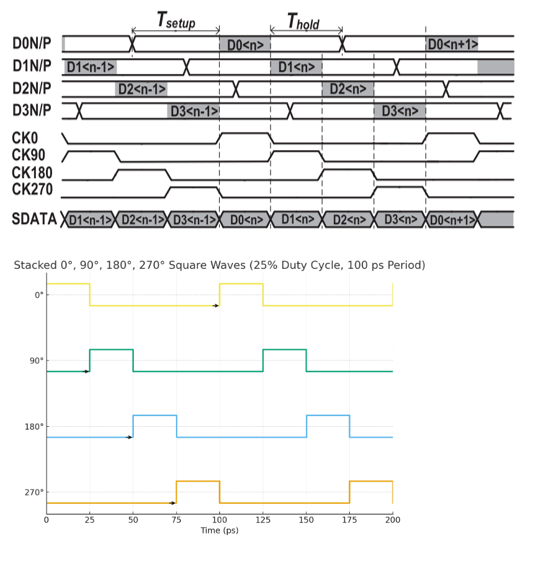
\includegraphics[width=0.8\textwidth]{img/TX_img/core idea.png}
    \caption{Timing diagram of the Quarter-Rate serialization scheme. The lower waveforms depict the proposed 25\% duty cycle clock phases ($0^\circ, 90^\circ, 180^\circ, 270^\circ$), which create strictly non-overlapping selection windows to sequentially serialize the parallel input data ($D_0-D_3$) without signal contention.}
    \label{fig:quarter_rate_timing}
\end{figure}

% =========================================================
% REVISED LITERATURE REVIEW (Neutral & Professional)
% =========================================================
\section{Literature Review of Multiplexer Topologies}

The design of the final 4:1 multiplexer stage is critical for signal integrity. Over the past decade, three primary circuit topologies have dominated the literature for high-speed serialization: Transmission Gates (TG), Current-Mode Logic (CML), and CMOS Tri-State Logic. This section surveys their operating principles and performance trade-offs in the context of high-speed PAM4 signaling.

\clearpage

\subsection{Transmission Gate (TG) based Topology}
The CMOS Transmission Gate (TG) functions as a high-speed passive switch, utilizing parallel NMOS and PMOS devices to pass the signal from input to output.

\begin{figure}[H]
    \centering
    % REPLACE 'piso.jpg' with your filename
    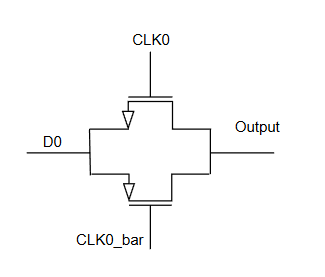
\includegraphics[width=0.5\textwidth]{img/TX_img/tg.png}
    \caption{Simple Schematic diagram of a CMOS Transmission Gate (TG) switch used in high-speed multiplexers.}
    \label{fig:tg_schematic}
\end{figure}

\begin{itemize}
    \item \textbf{Advantages:} The primary appeal of the TG topology is its zero static power consumption. Since it contains no direct path from supply to ground, it is theoretically the most power-efficient architecture for low-frequency applications.
    \item \textbf{Limitations:} As reviewed in recent literature, TG-based muxes face severe challenges at high data rates . The "Self-Loading" effect becomes dominant: to reduce the on-resistance ($R_{on}$), the transistor width must be increased, which inevitably increases the parasitic capacitance ($C_{par}$). This creates a fundamental bandwidth limit.
\end{itemize}
\newpage
\subsection{Current-Mode Logic (CML) based Topology}
Current-Mode Logic (CML) relies on Data an clock logical combination to generate the output.
\begin{figure}[H]
    \centering
    % REPLACE 'piso.jpg' with your filename
    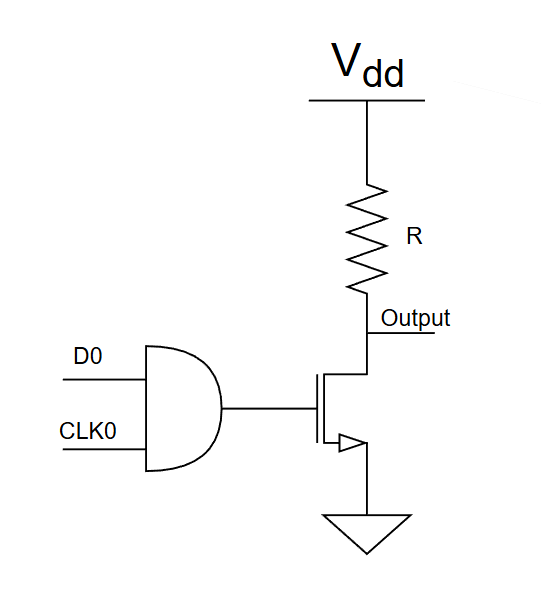
\includegraphics[width=0.5\textwidth]{img/TX_img/cml slice.png}
    \caption{Schematic of a Current-Mode Logic (CML) driver stage with a resistive load. In this implementation, the data ($D_0$) is logically combined with the clock ($CLK_0$) to gate the NMOS driver, allowing current to passthrough the load resistor $R$ only during the active phase.}
    \label{fig:cml_schematic}
\end{figure}
\begin{itemize}
    \item \textbf{Advantages:} CML is widely regarded in literature as the fastest logic family. Its differential nature provides excellent common-mode noise rejection, and its low voltage swing enables extremely fast switching speeds, making it a standard choice for optical and 100G+ interfaces.
    \item \textbf{Limitations:} The major drawback of CML is its high static power consumption, which occurs even when the data is not switching. Furthermore, the output swing is limited by the $I_{tail} \times R_{load}$ product. Achieving a high swing for acceptable SNR requires a large tail current or large load resistors, both of which degrade the power-bandwidth trade-off.
\end{itemize}
\newpage
\subsection{Active Tri-State Inverter based Topology}
The Tri-State inverter topology utilizes a clocked inverter structure (a stack of series transistors) to actively drive the output node.
\begin{figure}[H]
    \centering
    % Keeping the size consistent with the CML figure
    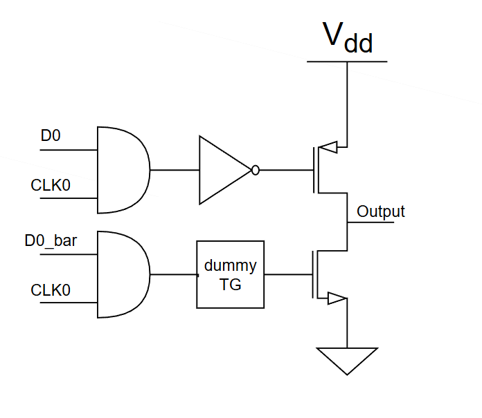
\includegraphics[width=0.5\textwidth]{img/TX_img/tri_slice.png}
    
    \caption{Schematic implementation of the Active Tri-State Inverter branch. The data inputs ($D_0$ and $\overline{D_0}$) are logically AND-ed with the clock phase ($CLK_0$). This ensures that both the PMOS and NMOS transistors are turned OFF (High-Impedance state) when the clock is inactive, preventing contention with other branches.}
    \label{fig:tristate_schematic_implementation}
\end{figure}

\begin{itemize}
    \item \textbf{Advantages:} Unlike the TG, the Tri-State topology is "active," meaning it regenerates the signal levels. This allows for a full rail-to-rail voltage swing, which maximizes the vertical and horizontal eye opening and.
    \item \textbf{Limitations:} The primary challenge documented in literature is Dynamic Power consumption. Since power scales with $CV^2f$, driving a full-swing signal at 64 Gb/s results in significant dynamic energy dissipation. Additionally, this topology is susceptible to "shoot-through" current (short-circuit power) during the brief moments when both PMOS and NMOS networks are partially on, requiring precise timing control of the clock phases.
\end{itemize}
\newpage
% =========================================================
% SECTION 2.3: SELECTION & ANALYSIS
% =========================================================
\section{Architecture Selection and Comparative Analysis}
\label{sec:arch_selection}

Following the review of available topologies, this section presents a comparative analysis based on the critical metrics for a 64 Gb/s PAM4 transmitter: Bandwidth, Power Consumption, jitter and Output Swing.

\subsection{Comparative Performance Metrics}
Table \ref{tab:topology_comparison} summarizes the trade-offs between the Transmission Gate (TG), Current-Mode Logic (CML), and Active Tri-State Inverter topologies based on recent literature in 22nm and similar nodes.

\begin{table}[htbp]
    \centering
    \caption{Comparative Analysis of Multiplexer Topologies for High-Speed SerDes}
    \label{tab:topology_comparison}
    \renewcommand{\arraystretch}{1.3} % Adds spacing to rows
    
    % The \resizebox command forces the table to fit exactly in the text width
    \resizebox{\textwidth}{!}{%
        \begin{tabular}{|l|c|c|c|}
        \hline
        \textbf{Metric} & \textbf{Transmission Gate (TG)} & \textbf{Current-Mode Logic (CML)} & \textbf{Tri-State Inverter} \\ \hline
        \textbf{Bandwidth} & Moderate & Very High & High \\ \hline
        \textbf{Static Power} & Zero (Leakage only) & High (Constant Tail Current) & Zero (Leakage only) \\ \hline
        \textbf{Dynamic Power} & Low & Low & High ($CV^2f$) \\ \hline
        \textbf{Output Swing} & Rail-to-Rail ($V_{DD}$) & Limited ($I \times R$) & Rail-to-Rail ($V_{DD}$) \\ \hline
        \textbf{Design Complexity} & Simple & Moderate & Moderate (Timing critical) \\ \hline
        \end{tabular}%
    }
\end{table}




\newpage
%%%%%%%%%%%  DRIVER  %%%%%%%%%%%%%%%%%%%%%%%%%%%
\section{The Function of the Driver} \label{sec:driver_function}
The most challenging building block in TX design is typically the line driver as it faces the most difficult demands of the standard: it must deliver high current levels to the channel while meeting the bandwidth requirements and maintaining signal integrity.

\subsection{Signal Integrity} \label{subsec:signal_integrity}
A driver with good signal integrity must successfully generate a signal with:

\begin{tasks}[label=$\bullet$, column-sep=10pt](2) % The (2) creates two columns
    \task High bit rate
    \task Low power consumption
    \task Low noise
    \task Free of unnecessary time domain spikes
    \task Precise $50\,\Omega$ impedance matching to prevent reflections
    \task High linearity to maintain uniform PAM-4 eye levels (RLM)
    \task Compensation for channel-induced Inter-Symbol Interference (ISI) through equalization
\end{tasks}
A useful visualization of signal integrity is the \textbf{eye diagram}
\subsection{Termination} \label{subsec:termination}
\begin{itemize}
    \item \textbf{Poly resistors} are typically used due to better linearity, but they typically vary $\pm 30\%$ over process and temperature. To mitigate this, control loops can be implemented for calibration. 
    \item \textbf{Active terminations} can also be utilized and programmed digitally; however, they lack robust Electrostatic Discharge (ESD) protection. By mixing and matching active and passive termination, a balance of better ESD robustness and high linearity is achieved. Furthermore, device capacitances are partially shielded in this configuration, preventing them from loading the output.
\end{itemize}

% --- First Image: Active Termination ---
\begin{figure}[htbp]
    \centering
    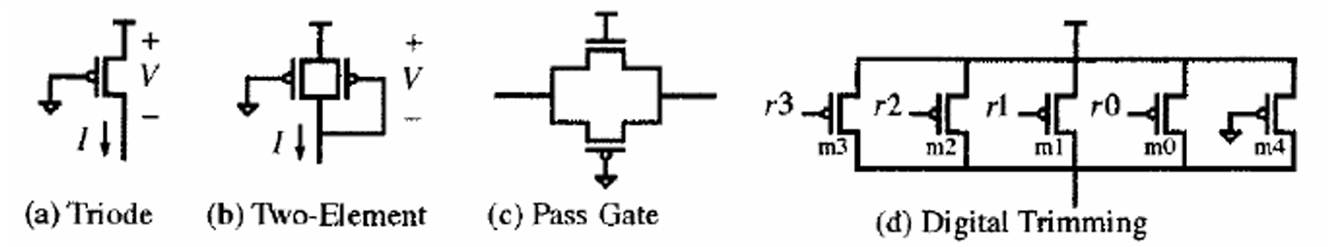
\includegraphics[width=0.9\linewidth]{img/TX_img/1)active_termination.png}
    \caption{Active termination}
    \label{fig:active_term}
\end{figure}

% --- Second Image: Combination ---
\begin{figure}[htbp]
    \centering
    
\includegraphics[width=0.4\linewidth]{2)combined_termination.png}
    \caption{Combination of Active and Passive}
    \label{fig:combined_term}
\end{figure}

\subsection{Equalization} \label{subsec:equalization}
\begin{itemize}
\item Equalization goal is to flatten the frequency response out to the Nyquist Frequency and remove time-domain ISI. TXs use pre-emphasis to shape their output spectrum (e.g., boosting high-frequency or de-emphasizing low-frequency content) , We usually use \textbf{de-emphasis} to not to increase Swing because we are limited by supply , EMI which will cause cross-talk , but at the cost of attenuated transmit signal

\item The number of taps and maximum tap weights determine allowable de-emphasis value and the quality of equalization both are usually specified by standards as more equalization , attenuates signal at small
frequency , so we limit this equalization because I have minimum eye opening

\item One approach to set the TX FIR coefficients is a \textbf{Minimum Mean-Square Error (MMSE) Algorithm}
\end{itemize}

\begin{figure}[htbp]
    \centering
    % 1. The Photo First
    
\includegraphics[width=0.5\textwidth]{3)Tx_FFE_Implementation.png}
    
    \vspace{10pt} 
    
    % 2. Mathematical representation exactly as requested
    \begin{center}
        \textbf{Low Frequency Response (Sum Taps)} \\
        $[\dots \enspace 1 \enspace 1 \enspace 1 \enspace \dots] * [-0.131 \enspace 0.595 \enspace -0.274] = [\dots \enspace 0.190 \enspace 0.190 \enspace 0.190 \enspace \dots]$ \\[10pt]
        \textbf{Nyquist Frequency Response (Sum Taps w/ Alternating Polarity)} \\
        $[\dots \enspace -1 \enspace 1 \enspace -1 \enspace \dots] * [-0.131 \enspace 0.595 \enspace -0.274] = [\dots \enspace 1 \enspace -1 \enspace 1 \enspace \dots]$
    \end{center}
    
    \vspace{5pt}
    
    % 3. The Caption at the very end
    \caption{Tx FFE Example}
    \label{fig:tx_ffe_example}
\end{figure}

\begin{figure}[H]
    \centering
    % --- Subfigure (a) ---
    \begin{subfigure}{0.32\textwidth}
        \centering
        
\includegraphics[width=\textwidth]{4.1)Channel_frequency_response.png}
        \caption{}
        \label{fig:channel_response}
    \end{subfigure}
    \hfill
    % --- Subfigure (b) ---
    \begin{subfigure}{0.32\textwidth}
        \centering
        
\includegraphics[width=\textwidth]{4.2)FIR_frequency_response.png}
        \caption{}
        \label{fig:fir_response}
    \end{subfigure}
    \hfill
    % --- Subfigure (c) ---
    \begin{subfigure}{0.32\textwidth}
        \centering
        
\includegraphics[width=\textwidth]{4.3)Combined_channel_and_Tx.png}
        \caption{}
        \label{fig:combined_response}
    \end{subfigure}

    \vspace{0.3cm}
    \caption{ (a) Channel frequency response ; (b) FIR frequency response ; (c) Combined channel and Tx}
    \label{fig:equalization_plots}
\end{figure}

\begin{figure}[H]
    \centering
    
\includegraphics[width=1\textwidth ]{5)sent_data.png}
    \caption{(a) Tx and Rx signals with lossy channel without Tx EQ; (b) Tx Pre-distorted output to compensate for channel ISI; (c) Rx received signal with Tx EQ}
    \label{fig:sent_data}
\end{figure}

\begin{itemize}
\item If no Tx pre-emphasis is used the single bit transitions are heavily attenuated compared to CIDs
\item When Tx pre-emphasis is used the transition bits are emphasized, non transition but are not emphasized
\item The channel attenuates the transition bits more than the non transition bits due to their higher frequency content
\item At the receiver input both transition and non transition bits have the same amplitude, i.e. ISI is eliminated
\end{itemize}

\begin{figure}[H]
    \centering
    
\includegraphics[width=1\textwidth ]{6)EYE.png}
    \caption{(a) RX eye diagram with lossy channel without Tx EQ; (b) Tx output eye diagram with pre-emphasis (pre-distorted eye); (c) Rx received eye diagram with Tx pre-emphasis}
    \label{fig:EYE}
\end{figure}

\begin{itemize}
\item Receiver eye was nearly closed without using Tx pre-emphasis resulting in high BER
\item After applying the right amount of pre-emphasis, ISI can be eliminated from the received eye
\item However, pre-emphasis also reduces the outer eye opening, i.e. the non 
transition bits are de-emphasized, thus a maximum limit is usually set by 
standards on how much pre-emphasis can be used

\end{itemize}
\newpage
\section{Analog-based and DAC-based Drivers} \label{sec:Analog/DAC-based}

The implementation of Feed-Forward Equalization (FFE) generally falls into two categories based on how the tap summation and signal modulation are performed.

\subsection{Analog-based transmitters} \label{subsec:Analog-based}
In analog-based transmitters, the equalization is performed by summing currents or voltages of the taps directly at the output node.

\begin{itemize}
    \item \textbf{Implementation Idea:} Tap weights are implemented by adjusting the number of active slices for each cursor (Pre, Main, and Post).
    \item \textbf{FFE Taps and Clocking:} To achieve UI-spaced FFE taps, custom digital delay elements such as latches are required. For tap programmability, high-speed MUXs clocked with multiple phases (half- or quarter-rate) are necessary. This significantly increases the complexity of the clocking tree and the capacitive load, often forcing equalization and tap selection to be handled at higher speeds.
    \item \textbf{Modulation Challenges:} Supporting higher modulation techniques, such as PAM-4, requires multiple serializers (e.g., separate paths for MSB and LSB) for a single cursor. This increases the capacitive loading on the transmitter output, which degrades the output bandwidth and significantly increases power consumption and complexity as the number of taps grows.
\end{itemize}


 \begin{figure}[htbp]
     \centering
     
\includegraphics[width=0.8\textwidth]{7)Analog-based}
     \caption{Analog-based Transmitter Architecture.}
 \end{figure}

\subsection{DAC-based transmitters} \label{subsec:DAC-based}
DAC-based transmitters move the equalization and tap weight calculation into the digital domain, using a Digital to Analog Converter (DAC) as the final output stage.
DAC-based architectures the dominant choice for TXs with five or more FFE taps

\begin{itemize}
    \item \textbf{Implementation Idea:} Equalization is performed digitally within a DSP. The DSP outputs a digital code representing the required analog voltage for each bit sent into the channel.
    \item \textbf{FFE Taps and Clocking:} Both the generation of taps and their programmability are handled in the digital domain. This eliminates the need for high-speed analog delay elements or high-speed MUXs for tap selection. Consequently, the pre-driver circuitry is much simpler, and the load on the clocking distribution is reduced , helping equalization and tap selection to be handled at lower speeds .
    \item \textbf{Modulation Flexibility:} The driver functions as a DAC that represents the weight of the bit code. This structure remains the same regardless of the modulation technique used. This architecture offers superior flexibility for supporting advanced modulation schemes like PAM-4 or PAM-8 without the massive complexity scaling seen in analog designs.
\end{itemize}


\begin{figure}[htbp]
     \centering
     
\includegraphics[width=0.8\textwidth]{8)DAC_Based}
     \caption{DAC-based Transmitter Architecture.}
 \end{figure}

 \subsubsection{Digital TX FFE} \label{ssubsec:DSP}

Digital TX FFEs are often implemented using Look-Up Tables (LUTs). A fully LUT-based implementation stores an $N$-tap filter span computation in an LUT, which requires an $N \cdot \log_2(M)$-bit address (for $M$-PAM modulation) and an output word width equal to the DAC resolution.

\begin{itemize}
    \item  For example, as shown in Fig.~\ref{fig:dac_ffe_lut_full}, a 2-PAM 4-tap FFE with 6-bit DAC resolution requires 16 rows and 6 columns, totaling 96 registers or memory cells. However, this architecture does not scale well for 4-PAM systems; a 7-tap FFE with 7-bit resolution would require $2^{14} \times 7 = 114,688$ registers.
    
    \item  Instead, a more efficient 4-PAM architecture, illustrated in Fig.~\ref{fig:dac_ffe_lut_per_tap}, uses per-tap LUTs to eliminate multipliers and employs digital adders to combine the tap values. This approach allows for simple 4-row LUTs per tap.
    
    \item Given the dramatic reduction in row count, the internal DSP resolution can be increased to 8 bits. This reduces quantization noise in the subsequent adders before the signal is finally quantized to the 7-bit DAC resolution.
    
    \item Using this per-tap approach, a 4-PAM 7-tap FFE can be implemented with only 224 registers ($7 \text{ taps} \times 4 \text{ rows} \times 8 \text{ bits}$), making it much more hardware-efficient.
\end{itemize}

\begin{figure}[htbp]
    \centering
    % --- Subfigure A ---
    \begin{subfigure}{0.35\textwidth} % Increased slightly for better visibility
        \centering
        
\includegraphics[width=\textwidth]{9)DAC_FFE_1.png}
        \caption{}
        \label{fig:dac_ffe_lut_full}
    \end{subfigure}
    \hfill % This pushes (a) to the left and (b) to the right
    % --- Subfigure B ---
    \begin{subfigure}{0.6\textwidth} % Adjusted to fill the remaining space
        \centering
        
\includegraphics[width=\textwidth]{9)DAC_FFE_2.png}
        \caption{}
        \label{fig:dac_ffe_lut_per_tap}
    \end{subfigure}
    
    \vspace{0.3cm}
    \caption{Digital TX FFE implementations. (a) Fully LUT-based 2-PAM 4-tap FFE with 6b output resolution; (b) 4-PAM 7-tap FFE with tap-based LUTs and 7b output resolution.}
    \label{fig:dac_ffe_comparison}
\end{figure}
The reduction in register count is driven by the mathematical difference between \textbf{exponential growth} and \textbf{linear growth} as the number of taps ($N$) increases.

In the standard approach, a 7-tap 4-PAM system must account for every possible input combination ($4^7 = 16,384$ combinations) and gives the output directly. By treating each tap independently (multiplying each tap with its tap weight), the per-tap approach only needs to store 4 possible values for each of the 7 taps.
\begin{table}[htbp]
    \centering
    \caption{Comparison of the 2 Implementation Architectures}
    \label{tab:lut_comparison}
    \begin{tabular}{@{}lll@{}}
        \toprule
        \textbf{Feature} & \textbf{Fully LUT-Based Approach} & \textbf{Per-Tap LUT Approach} \\ \midrule
        Logic Basis & $2^{N \cdot \log_2(M)}$ rows & $M$ rows per tap \\
        Scaling for 4-PAM 7-Tap & Requires $2^{14}$ addresses & Requires $4$ rows $\times 7$ taps \\
        Total Registers & 114,688 registers & 224 registers \\ \bottomrule
    \end{tabular}
\end{table}

\section{Driver Topologies} \label{sec:Driver_topologies}
\subsection{Voltage Mode} \label{subsec:Voltage_mode}
\subsubsection{NRZ SST} \label{ssubsec:NRZ_SST}

\begin{figure}[H]
    \centering
    % --- Subfigure (a) ---
    \begin{subfigure}{0.4\linewidth}
        \centering
        
\includegraphics[width=\textwidth]{10)SST}
        \caption{}
        \label{fig:SST}
    \end{subfigure}
    \hfill
    % --- Subfigure (b) ---
    \begin{subfigure}{0.21\linewidth}
        \centering
        
\includegraphics[width=\textwidth]{10.1)Equivalent_Circuit}
        \caption{}
        \label{fig:Equivalent Circuit_NRZ}
    \end{subfigure}
    \hfill
    \vspace{0.3cm}
    \caption{ (a) SST ; (b) Equivalent Circuit}
    \label{fig:NRZ SST}
\end{figure}

\begin{itemize}
    \item SST driver consists of inverters driving series termination resistors.
    \item Actual source impedance is a series combination of $R_{TERM}$ and $Z_{NMOS}$ or $Z_{PMOS}$.
    \item The series resistors provide ESD protection for transistors’ drain junctions.
    \item Transistor impedance varies with region of operation and PVT corners.
    \item Differential peak-to-peak output swing is equal to $V_{DD}$.
\end{itemize}


\subsubsection{PAM-4 SST} \label{ssubsec:PAM-4_SST}

\begin{figure}[H]
    \centering
    % --- Top Row ---
    \begin{subfigure}[t]{0.48\linewidth} % Adjusted to fit side-by-side
        \centering
        
\includegraphics[width=\textwidth]{11)PAM4_SST}
        \caption{2-bit (PAM-4) SST Architecture}
        \label{fig:PAM4_SST_Circuit}
    \end{subfigure}
    \hfill % Pushes subfigures to the edges
    \begin{subfigure}[t]{0.48\linewidth} % Adjusted to fit side-by-side
        \centering
        
\includegraphics[width=\textwidth]{11.2)Equivalent_Circuit_PAM4}
        \caption{Equivalent Circuit}
        \label{fig:Equivalent_Circuit_PAM4}
    \end{subfigure}

    \vspace{0.5cm} % Adds vertical space before the next row

    % --- Bottom Row (A blank line above this forces it down) ---
    \begin{subfigure}[t]{0.6\linewidth} % Larger width for the centered EYE
        \centering
        
\includegraphics[width=\textwidth]{11.3)EYE}
        \caption{EYE Diagram}
        \label{fig:sttpam4eye}
    \end{subfigure}
    
    \caption{}
    \label{fig:PAM-4_SST_Main}
\end{figure}


\begin{itemize}
\item It can be Considered as a 2 bit DAC corresponding to 3 identical slices ($2^{n}-1$) 
\item So We want to make the resistance of all the parallel slices gives 50$\Omega$ so the resistance of one slice = 50X3 $\Omega$ and Width of each slice = 3*W wanted where the whole driver will have Width = W and R=50$\Omega$
\item Voltage divider is made for each input and for complementary input : the 2 terminals of Vout are swapped so for Vppd it will be the same with opposite sign
\end{itemize}
\newpage

\subsection{Current Mode} \label{subsec:Current_mode}
\subsubsection{NRZ CML} \label{ssubsec:NRZ_CML}
 \begin{figure}[H]
     \centering
     
\includegraphics[width=0.8\textwidth]{12)CML}
     \caption{Conventional CML.}
 \end{figure}
 \begin{itemize}
    \item Differential pair steers the current into a differential I/O link.
    \item Differential pp RX swing is \textbf{$\pm IR/2$.}
    \item Note that \textbf{Swing = IR} and \textbf{Vo,CM = VDD-IR/2}, so by ignoring supply variations, we can have precise Swing and CM by using I outputted from Bandgap which track $1/R$ and use poly resistor so If R shifted I will shift opposite to it So swing and CM become constant.
    \item For high swing (Large current) we will need large i/p pair to have lower $V_{GS}$ and preserve current source in Sat. For ex: $0.8V_{pp}$ swing needs $I_B=16mA$ (w/o taking current mirrors into considerations).
    \item So a pre-driver is necessary to drive the large capacitance of the output stage (chain of inverters).
    \item Tradeoffs between Power, speed, swing, BER.
\end{itemize}


\clearpage
\subsubsection{PAM-4 CML} \label{ssubsec:PAM-4_CML}
\begin{figure}[H]
    \centering
    % --- Top Row ---
    \begin{subfigure}[t]{0.48\linewidth} % Adjusted to fit side-by-side
        \centering
        
\includegraphics[width=\textwidth]{13)PAM4CML}
        \caption{2-bit (PAM-4) CML Architecture}
        \label{fig:PAM4_SST_Circuit}
    \end{subfigure}
    \hfill % Pushes subfigures to the edges
    \begin{subfigure}[t]{0.51\linewidth} % Adjusted to fit side-by-side
        \centering
        
\includegraphics[width=\textwidth]{13.1)Equiv_cir}
        \caption{Equivalent Circuit}
        \label{fig:Equivalent_Circuit_PAM4}
    \end{subfigure}

    \vspace{0.5cm} % Adds vertical space before the next row

    % --- Bottom Row (A blank line above this forces it down) ---
    \begin{subfigure}[t]{0.5\linewidth} % Larger width for the centered EYE
        \centering
        
\includegraphics[width=\textwidth]{13.2)EYE}
        \caption{EYE Diagram}
        \label{fig:sttpam4eye}
    \end{subfigure}
    
    \caption{}
    \label{fig:PAM-4_SST_Main}
\end{figure}
\noindent \textbf{For D<1:0>=10:} 

\begin{enumerate}
    \item \textbf{KCL at node $V_{on}$}:
    \begin{equation}
        \frac{V_{DD} - V_{on}}{R} + I_{2R} = \frac{2}{3}I \label{eq:kclnodevon10}
    \end{equation}
    
    \item \textbf{KCL at node $V_{op}$}:
    \begin{equation}
        \frac{V_{DD} - V_{op}}{R} - I_{2R} = \frac{1}{3}I \label{eq:kclnodevop10}
    \end{equation}
\end{enumerate}

Subtracting equation \eqref{eq:kclnodevop10} from equation \eqref{eq:kclnodevon10} yields:
\begin{equation}
    \frac{V_{op} - V_{on}}{R} + 2I_{2R} = \frac{1}{3}I
    \label{eq:substpam4cml}
\end{equation}

By Ohm's Law, the differential voltage is defined as $V_{op} - V_{on} = I_{2R}(2R)$ . Substituting this into equation \eqref{eq:substpam4cml}:
\begin{equation}
    \frac{2R \cdot I_{2R}}{R} + 2I_{2R} = \frac{1}{3}I
\end{equation}

\begin{equation}
    4I_{2R} = \frac{1}{3}I \implies I_{2R} = \frac{1}{12}I
\end{equation}

This result confirms that the current passing through the bridging resistor is exactly $1/12$ of the total tail current $I$ 
\begin{equation}
    V_{diff} = +\frac{1}{12}I \times 2R = +\frac{1}{6}IR 
     \label{eq:vout_final}
\end{equation}
\begin{align}
    V_{oN} &= V_{DD} - \frac{7}{12} IR \\
    V_{oP} &= V_{DD} - \frac{5}{12} IR
\end{align}
And for the Complementary input , for differential peak to peak , We know that it is just change in the direction of the current so Vppd is the same with opposite sign
\noindent \textbf{For D<1:0>=11:} 


\begin{equation}
    I_{2R} = \frac{1}{4}I_s
\end{equation}

The differential output voltage $V_{diff}$ is then calculated as:
\begin{equation}
    V_{diff} = I_{2R}(2R) = \left( \frac{1}{4}I_s \right)(2R) = \frac{1}{2}I_sR
\end{equation}
\begin{align}
    V_{oN} &= V_{DD} - \frac{3}{4} IR \\
    V_{oP} &= V_{DD} - \frac{1}{4} IR
\end{align}
\newpage
\subsubsection{H-bridge CML} \label{ssubsec:H_CML}

 \begin{figure}[H]
     \centering
     
\includegraphics[width=0.5\textwidth]{14)H-bridge}
     \caption{H-Bridge}
 \end{figure}
 \begin{itemize}
    \item \textbf{Output Swing Calculation}:  $V_{oPP,diff} = 2I_B R$ .
    \item \textbf{Power and Area Trade-offs}: Swing is doubled for the same power consumption but requires a larger circuit area . For the same swing as CML, we need $1/2$ the size of the NMOS input pair, but the addition of PMOS transistors with sizes larger than $1/2$ the area of the CML NMOS increases parasitic capacitance .
    \item \textbf{Headroom and Common-Mode (CM) Challenges}: The presence of two series current sources occupies a large voltage headroom . Furthermore, the output CM is not inherently defined; this can be resolved using a CMFB (Common-Mode Feedback) loop or by implementing a hybrid topology .
    \item \textbf{Hybrid Topology}: In a hybrid configuration, the SST defines the output CM, and the CML adds its swing on top of it; however, this approach increases self-loading .
\end{itemize}

\subsubsection{Tailless} \label{ssubsec:Tailless}
 \begin{figure}[H]
     \centering
     
\includegraphics[width=1\textwidth]{16)Tailless}
     \caption{Tailless}
 \end{figure}
The tailless driver architecture offers significant advantages for high-speed data transmission by optimizing the transistor biasing and reducing parasitic effects.

\begin{itemize}
    \item \textbf{Device Operation}: The tailless driver consists of switching and cascode transistors that are flipped from the input and tail current source used in standard CML drivers. This configuration requires only the cascode (Casc) devices to remain in the saturation region for proper operation and they are whom defines current and though swing.
    
    \item \textbf{Parasitic Reduction}: By eliminating the tail current source, the $V_{GS}$ of the input pair can be increased. This allows the driver to deliver the same current (and thus the same output swing) using a smaller input pair, which significantly decreases parasitic capacitance. However, a high overdrive voltage ($V_{OV}$) must be managed to prevent transistors from entering the linear region.
    
    \item \textbf{Device Protection}: The $V_{DS}$ of the switches is determined by the $V_{GS}$ of the cascode transistors. Applying an appropriate $V_{casc}$ protects the input transistors from large output swings, enabling the use of thin-oxide devices which are essential for achieving the final high data rate.
    
    \item \textbf{Current Control}: In specific configurations, the P1 in fig(b) can disable current flow in the driver by pulling the source of N1 to the supply voltage when the digital input ($DIN$) is low.
    
    \item \textbf{Output Impedance ($R_{out}$)}: The cascode transistors are the primary devices forcing current, typically requiring a high channel length ($L$). However, since they connect directly to the output, $L$ is kept small to avoid increasing parasitics. To compensate and boost $R_{out}$, a "super $g_m$" configuration is  in fig(c), which is further amplified by the loop gain ($LG$).
\end{itemize}

\subsection{Hybrid Mode} \label{subsec:Hybrid_mode}
\begin{itemize}
    \item Since V.mode max swing is VDD and CML high swings will give high non linearity , Hybrid topology is proposed to make the best compromise of them in addition to increasing the output swing above VDD
    \item For the corner @which supply decrease -10\% and 50mV routing so supply is 670mV , we will want 130mV additional swing from the CML to acheive the standard swing spec specified in table \ref{tab:pcie6_tx_specs_full} , so we will give margin and say we want 135mV swing
\end{itemize}

\subsubsection{NRZ NMOS CML}
\begin{figure}[H]
    \centering
    \begin{subfigure}{0.5\linewidth} % Use linewidth for the environment
        \centering
        
\includegraphics[width=\textwidth]{17.1)Hybrid_NMOS_CML}
        \caption{}
    \end{subfigure}
    \hfill
    \begin{subfigure}{0.6\linewidth} % Use linewidth for the environment
        \centering
        
\includegraphics[width=\textwidth]{17.1)Hybrid_NMOS_CML_EQ_CIRC}
        \caption{}
    \end{subfigure}
    \caption{(a) NRZ NMOS CML; (b) Equivalent Circuit.}
\end{figure}
\begin{itemize}
    \item The current distribution is only made by for I bas and VDD is deactivated (superposition) 
    \item This topology will give Vppd = VDD+IR
    \item It is obvious that this topology isn't suitable as VDS on Current source and Input is too low
    \item  Assuming for the corner that the supply is low (670mV) and we want IR=135mV so VoutP = 66.25mV which is bad headroom
\end{itemize}
 
\subsubsection{NRZ PMOS CML}
\begin{figure}[H]
    \centering
    \begin{subfigure}{0.5\linewidth} % Use linewidth for the environment
        \centering
        
\includegraphics[width=\textwidth]{17.2)Hybrid_PMOS_CML}
        \caption{}
    \end{subfigure}
    \hfill
    \begin{subfigure}{0.6\linewidth} % Use linewidth for the environment
        \centering
        
\includegraphics[width=\textwidth]{17.2)Hybrid_PMOS_CML_EQ_CIRC}
        \caption{}
    \end{subfigure}
    \caption{(a) NRZ PMOS CML; (b) Equivalent Circuit.}
\end{figure}
\begin{itemize}
    \item This topology will give Vppd = VDD+IR
    \item Same VDS as the prev topology and it is still unsuitable

\end{itemize}
\newpage
\subsubsection{NRZ H-bridge CML}
\begin{figure}[H]
    \centering
    \begin{subfigure}{0.5\linewidth} % Use linewidth for the environment
        \centering
        
\includegraphics[width=\textwidth]{17.3)Hybrid_HBridge_CML}
        \caption{}
    \end{subfigure}
    \hfill
    \begin{subfigure}{0.6\linewidth} % Use linewidth for the environment
        \centering
        
\includegraphics[width=\textwidth]{17.3)Hybrid_HBridge_CML_EQ_CIRC}
        \caption{}
        \label{fig:NRZ_HBRIDGECMLEQCIRC}
    \end{subfigure}
    \caption{(a) NRZ H-Bridge CML; (b) Equivalent Circuit.}
\end{figure}
\begin{itemize}
    \item This topology will give Vppd = VDD+2IR as the H-bridge topology made 1/2 of I bias pass through RX termination instead of 1/4Ibias
    \item It will give VDS = 133.75mV which is more suitable than the prev topologies but note that input pair will be in triode (|VG-VD| $\approx$ 666.25mV >|VTH| so this should be considered in Resistance calibration)

\end{itemize}
\newpage
\subsubsection{PAM-4 H-bridge CML}

\begin{figure}[H]
    \centering
    \begin{subfigure}{0.6\linewidth} % Use linewidth for the environment
        \centering
        
\includegraphics[width=\textwidth]{17)Hybrid}
        \caption{}
    \end{subfigure}
    \hfill
    \begin{subfigure}{0.7\linewidth} % Use linewidth for the environment
        \centering
        
\includegraphics[width=\textwidth]{17)HybridPAM4EQCIRC.png}
        \caption{}
        \label{}
    \end{subfigure}
    \caption{(a) Hybrid H-bridge Driver; (b) Equivalent Circuit for D<1:0> = 10.}
\end{figure}
\begin{itemize}
    \item For $D\langle 1:0 \rangle = 11, 00$: \newline 
    The equivalent circuit is the same as fig \ref{fig:NRZ_HBRIDGECMLEQCIRC} and 
    $\bm{V_{ppd} = V_{DD} + 2RI = V_{DD} + \Delta V}$
\item For $D\langle 1:0 \rangle = 10, 01$:
\begin{align*}
    % Top line: Entire equation is bold, but "where" is standard weight
    \pmb{V_{ppd}} &\pmb{= \frac{V_{DD}}{3} + \frac{2RI}{3} = \frac{V_{DD}}{3} + \frac{\Delta V}{3},} \quad \text{where } \pmb{\Delta I = \frac{I}{3}} \\
    % Lower lines: Return to standard weight
    V_{DS(I_{LSB})} &= \frac{7}{12} V_{DD} + \frac{1}{2} R \Delta I = 509.6 \text{ mV} \\
    V_{DS(I_{MSB})} &= \frac{5}{12} V_{DD} - \frac{1}{2} R \Delta I = 269 \text{ mV}
\end{align*}


\end{itemize}
\subsection{Comparisons} \label{subsec:comp}
\subsubsection{Power} \label{ssubsec:Power}
\begin{figure}[H]
     \centering
     
\includegraphics[width=0.7\textwidth]{18.1)powercml}
     \caption{}
 \end{figure}
 \begin{figure}[H]
     \centering
     
\includegraphics[width=0.7\textwidth]{18.2)powersst}
     \caption{}
 \end{figure}
 \clearpage
 
 \subsubsection{Swing} \label{ssubsec:Swing}
\begin{figure}[H]
    \centering
    % --- Subfigure A ---
    \begin{subfigure}{0.65\textwidth} % Increased slightly for better visibility
        \centering
        
\includegraphics[width=\textwidth]{15)comp1}
        \caption{}
        \label{}
    \end{subfigure}
    \hfill % This pushes (a) to the left and (b) to the right
    % --- Subfigure B ---
    \begin{subfigure}{0.6\textwidth} % Adjusted to fill the remaining space
        \centering
        
\includegraphics[width=\textwidth]{15)comp2}
        \caption{}
        \label{}
    \end{subfigure}
    
    \vspace{0.3cm}
    \caption{CML Swings for SE termination. (a) CML; (b) H-bridge.}
    \label{fig:dac_ffe_comparison}
\end{figure}
\noindent \textbf{For CML : }
Total current is passing in one branch
\noindent \textbf{For H-Bridge :}
Total Current is passing in each of the 2 branches
• Current is divided equally between TX termination and RX termination
• ½  of the current reached to each SE  termination of the receiver
\begin{figure}[H]
    \centering
    % --- Subfigure A ---
    \begin{subfigure}{0.65\textwidth} % Increased slightly for better visibility
        \centering
        
\includegraphics[width=\textwidth]{15)comp3}
        \caption{}
        \label{}
    \end{subfigure}
    \hfill % This pushes (a) to the left and (b) to the right
    % --- Subfigure B ---
    \begin{subfigure}{0.65\textwidth} % Adjusted to fill the remaining space
        \centering
        
\includegraphics[width=\textwidth]{15)comp4}
        \caption{}
        \label{}
    \end{subfigure}
    
    \vspace{0.3cm}
    \caption{CML Swings for Differential termination. (a) CML; (b) H-bridge.}
    \label{}
\end{figure}

\noindent \textbf{For CML : }
\begin{itemize}
    \item at D=VDD , Db=0 :
    \begin{align}
        V_1 &= V_{DD} - \frac{3}{4} I_b R_T \\
        V_2 &= V_{DD} - \frac{1}{4} I_b R_T
    \end{align}
    \item ¼ of the current reached the differential Termination of the receiver
    \item The 2nd termination of TX became series with RX termination
\end{itemize}
\noindent \textbf{For H-Bridge :}
Total Current is passing in each of the 2 branches
• Current is divided equally between TX termination and RX termination
• ½  of the current reached the differential Termination of the receiver
 \begin{figure}[H]
     \centering
     
\includegraphics[width=1\linewidth]{10.2)Swings}
     \caption{ SST Swings a) SE Termination ; b) Differential Termination}
 \end{figure}
 
\noindent \textbf{For SE termination:}
\begin{align}
    V_{d,1} &= (Vs/2) & V_{d,0} &= -(Vs/2) \\
    V_{d,pp} &= Vs & I &= \frac{V_{d,pp}}{2R}              
\end{align}

\vspace{0.5cm}

\noindent \textbf{For Differential termination:}
\begin{align}
    V_{d,1} &= (Vs/2) & V_{d,0} &= -(Vs/2) \\
    V_{d,pp} &= Vs & I &= \frac{V_{d,pp}}{4R}     
\end{align}
\clearpage
 \subsubsection{Summary} \label{ssubsec:Summary}
\begin{table}[htbp]
    \centering
    \caption{Comparison Between Current Mode and Voltage Mode Driver Topologies}
    \label{tab:driver_comparison}
    \begin{tabularx}{\textwidth}{l X X}
        \toprule
        \textbf{Feature} & \textbf{Current Mode} & \textbf{Voltage Mode} \\
        \midrule
        \textbf{Swing} & Swing is set by current . & Swing is set by Supply. \\
        \addlinespace
        \textbf{Termination} & termination is set by $Z_0$ at high $R_{out}$. &  termination set by $Z_0$ and devices. \\
        \addlinespace
        \textbf{Power} & Static power; Less power efficient for same swing. & Dynamic power;  but for high speed , the very fast transitions can be averaged to be compared with static current,  more power efficient for same swing. \\
        \addlinespace
        \textbf{Speed} & faster due to constant current source activation  &  it is slower as it depends on charging and discharging caps \\        

        \addlinespace
        \textbf{SSO} & Static steered current prevents fast transitions. & Fast transitions can lead to supply bounce if parasitic inductors are present. \\
        \addlinespace
        \textbf{Programmability} & Swing is analog-programmed via current source without altering driver impedance. & Harder termination controllability ($R_{ON}$ depends on $\mu, V_{th}$, etc.). Analog Tuning through header/footer CSs degrades linearity. \\
        \addlinespace
        \textbf{Linearity} & Degraded linearity as current source operates in different regions during transitions. & Better linearity; series resistance overcomes $R_{ON}$ non-linearity. \\
        \addlinespace
        \textbf{Trade-offs} & Swing $\uparrow$, $V_{oCM} \downarrow$, headroom $\downarrow$, linearity $\downarrow$ (tail operates close to triode). Input size $\uparrow$, headroom for tail $\uparrow$, BW $\downarrow$. & Linearity vs. Speed trade-off. Increasing $Z_0/R_{ON}$ improves linearity but degrades bandwidth (BW). \\
        \bottomrule
    \end{tabularx}
\end{table}
